\documentclass{article}
\usepackage{neurips_2026}
\usepackage[utf8]{inputenc}
\usepackage[T1]{fontenc}
\usepackage{hyperref}
\usepackage{url}
\usepackage{booktabs}
\usepackage{amsfonts,amsmath,amssymb,amsthm}
\usepackage{nicefrac}
\usepackage{microtype}
\usepackage{graphicx}
\usepackage{float}
\usepackage{xcolor}
\graphicspath{{../figures/}}
% generated by paper/scripts/make_numbers.py from results/; do not edit
\newcommand{\EoneOLSA}{0.86}
\newcommand{\EoneDMA}{0.51}
\newcommand{\EoneOLSB}{0.46}
\newcommand{\EoneDMB}{0.50}
\newcommand{\EoneOLSC}{0.21}
\newcommand{\EoneDMC}{0.50}
\newcommand{\EoneSlope}{-0.51}
\newcommand{\EoneBiasMax}{0.009}
\newcommand{\EoneDMbias}{-0.50}
\newcommand{\EoneTwohopA}{1.05}
\newcommand{\EthreeOLSZ}{0.72}
\newcommand{\EthreeDMZ}{0.06}
\newcommand{\EthreeOLSH}{0.46}
\newcommand{\EthreeDMH}{0.34}
\newcommand{\EthreeOLSO}{0.35}
\newcommand{\EthreeDMO}{0.50}
\newcommand{\EthreeOLSF}{0.13}
\newcommand{\EthreeDMF}{0.80}
\newcommand{\EthreeCntZ}{2.17}
\newcommand{\EtwoSbmLo}{0.09}
\newcommand{\EtwoSbmHi}{2.51}
\newcommand{\EtwoErLo}{0.08}
\newcommand{\EtwoErHi}{0.43}
\newcommand{\EnineCzero}{0.12}
\newcommand{\EnineCthree}{0.98}
\newcommand{\CovClMin}{0.85}
\newcommand{\CovClMax}{0.94}
\newcommand{\CovHcMin}{0.50}
\newcommand{\CovClSbmN}{0.94}
\newcommand{\CovClSbmSmall}{0.88}
\newcommand{\CovHcSbmMix}{0.73}
\newcommand{\EsevenLinAOls}{0.20}
\newcommand{\EsevenLinAGbm}{0.56}
\newcommand{\EsevenLinARidge}{0.94}
\newcommand{\EsevenLinACub}{0.29}
\newcommand{\EsevenBiasLinAOls}{-0.01}
\newcommand{\EsevenBiasLinAGbm}{-0.06}
\newcommand{\EsevenLinBOls}{0.68}
\newcommand{\EsevenLinBGbm}{0.76}
\newcommand{\EsevenLinBRidge}{2.24}
\newcommand{\EsevenLinBCub}{3.51}
\newcommand{\EsevenBiasLinBOls}{+0.01}
\newcommand{\EsevenBiasLinBGbm}{-0.31}
\newcommand{\EsevenThrAOls}{0.40}
\newcommand{\EsevenThrAGbm}{0.56}
\newcommand{\EsevenThrARidge}{1.03}
\newcommand{\EsevenThrACub}{0.29}
\newcommand{\EsevenBiasThrAOls}{+0.35}
\newcommand{\EsevenBiasThrAGbm}{+0.02}
\newcommand{\EsevenThrBOls}{0.95}
\newcommand{\EsevenThrBGbm}{0.73}
\newcommand{\EsevenThrBRidge}{2.42}
\newcommand{\EsevenThrBCub}{3.73}
\newcommand{\EsevenBiasThrBOls}{+0.64}
\newcommand{\EsevenBiasThrBGbm}{-0.13}
\newcommand{\EsixCntEr}{1.97}
\newcommand{\EsixCntErFrac}{1.65}
\newcommand{\EsixCntAdjEr}{0.28}
\newcommand{\EsixCntAdjErFrac}{0.29}
\newcommand{\EsixTwohopBias}{-0.23}
\newcommand{\EsixCntAdjBaBias}{-0.41}
\newcommand{\MainOneOls}{0.19}
\newcommand{\MainDM}{0.50}
\newcommand{\MainThreeBernLow}{0.63}
\newcommand{\MainThreeBernLowBias}{+0.53}
\newcommand{\MainFourBias}{-0.22}
\newcommand{\MainFourTwohopBias}{+0.01}
\newcommand{\MainEgoOls}{0.34}
\newcommand{\MainStanOls}{0.10}
\newcommand{\HajekUndefBernHalf}{0.01}
\newcommand{\HajekUndefBernLow}{0.99}
\newcommand{\NMainCells}{72}
\newcommand{\HsevenSat}{0.87}
\newcommand{\HsevenPooled}{0.42}
\newcommand{\HsevenThresh}{0.05}
\newcommand{\HsevenPow}{0.15}
\newcommand{\HsevenHet}{0.00}
\newcommand{\TheoryVarMed}{1.008}
\newcommand{\TheoryVarLo}{0.977}
\newcommand{\TheoryVarHi}{1.039}
\newcommand{\TheoryVarN}{496}
\newcommand{\TheoryBiasN}{626}
\newcommand{\TheoryBiasCorr}{0.99998}
\newcommand{\TheoryBiasMaxDiff}{0.081}
\newcommand{\EelevenSbmBias}{-0.26}
\newcommand{\EelevenSbmGOne}{0.31}
\newcommand{\EelevenWeakOls}{0.38}
\newcommand{\EelevenWeakDM}{0.21}
\newcommand{\CovHcSbmLoA}{0.56}
\newcommand{\CovHcSbmLoB}{0.50}
\newcommand{\CovHcSbmMixB}{0.65}
\newcommand{\CovClBaA}{0.90}
\newcommand{\CovClBaB}{0.85}
\newcommand{\CovClSbmMixA}{0.88}
\newcommand{\CovClSbmMixB}{0.93}
\newcommand{\EelevenSbmZero}{0.21}
\newcommand{\EelevenSbmGOneDM}{0.50}
\newcommand{\EelevenEgoBias}{-0.27}
\newcommand{\EelevenEgoGOne}{0.43}
\newcommand{\EelevenEgoZero}{0.46}
\newcommand{\HsevenClSat}{0.89}
\newcommand{\HsevenClTwohop}{0.99}
\newcommand{\HsevenClHet}{0.68}
\newcommand{\HsevenBernTwohop}{0.00}
\newcommand{\MainOlsEr}{0.14}
\newcommand{\MainOlsBa}{0.14}
\newcommand{\MainOlsSbm}{0.25}
\newcommand{\MainOlsWs}{0.25}
\newcommand{\MainTwohopOneSbm}{1.30}
\newcommand{\MainTwohopOneEgo}{0.87}
\newcommand{\MainTwohopOneStan}{0.72}
\newcommand{\MainDMmedBernHalf}{0.50}
\newcommand{\MainDMmedCluster}{0.27}
\newcommand{\MainDMClOne}{0.27}
\newcommand{\MainOlsClOne}{0.18}
\newcommand{\MainDMClThree}{0.31}
\newcommand{\MainOlsClThree}{0.17}
\newcommand{\MainDMClFour}{0.33}
\newcommand{\MainOlsClFour}{0.22}
\newcommand{\MainDMClFive}{0.31}
\newcommand{\MainOlsClFive}{0.18}
\newcommand{\MainFourBiasCl}{-0.06}
\newcommand{\EfiveBetterN}{9}
\newcommand{\EfiveLo}{0.11}
\newcommand{\EfiveHi}{0.34}
\newcommand{\EfiveEgo}{0.55}
\newcommand{\EfiveEr}{0.13}
\newcommand{\EfiveSbmLo}{0.34}
\newcommand{\EfiveSbmMid}{0.23}
\newcommand{\EthreeSdLo}{0.62}
\newcommand{\EthreeSdHi}{0.76}
\newcommand{\EfourPowLo}{+0.44}
\newcommand{\EfourPowHi}{-0.23}
\newcommand{\EfourQuadLo}{-0.34}
\newcommand{\EfourQuadMid}{0.00}
\newcommand{\EfourQuadHi}{+0.34}
\newcommand{\EfourThrLoDten}{-0.27}
\newcommand{\EfourThrMidDten}{+0.34}
\newcommand{\EfourThrHiDten}{-0.30}
\newcommand{\EfourThrMidDhund}{+0.71}
\newcommand{\RdEgoOneMean}{0.43}
\newcommand{\RdEgoOneLo}{0.27}
\newcommand{\RdEgoOneHi}{0.65}
\newcommand{\RdEgoOneSd}{0.11}
\newcommand{\RdEgoOneDM}{0.50}
\newcommand{\RdEgoWinsHalf}{21}
\newcommand{\RdEgoWinsTenth}{1}
\newcommand{\RdEgoWinsCl}{10}
\newcommand{\RdEgoThreeHalf}{4}
\newcommand{\RdEgoFiveHalf}{2}
\newcommand{\RdStanOneMean}{0.12}
\newcommand{\RdStanOneLo}{0.09}
\newcommand{\RdStanOneHi}{0.16}
\newcommand{\RdStanOneSd}{0.03}
\newcommand{\RdStanOneDM}{0.50}
\newcommand{\RdStanWinsHalf}{32}
\newcommand{\RdStanWinsTenth}{31}
\newcommand{\RdStanWinsCl}{15}
\newcommand{\RdStanThreeHalf}{8}
\newcommand{\RdStanFiveHalf}{8}


\newcommand{\gate}{\tau}
\newcommand{\E}{\mathbb{E}}
\newcommand{\bz}{\mathbf{z}}

\title{How Accurate Is Regression Adjustment for the Global Treatment Effect Under Network Interference?}
\author{Anonymous Authors}

\begin{document}
\maketitle

\begin{abstract}
Regression adjustment, which regresses outcomes on a unit's own treatment and a summary of its neighbours' treatments and then predicts under all-treated and all-control, is a common way to estimate the global average treatment effect (GATE) under network interference, but little is known about how accurate it is or what limits it. We study it on synthetic outcomes with an exactly known GATE on four synthetic graph families and two public Facebook graphs, over 72 main-grid cells (graphs $\times$ interference mechanisms $\times$ designs) and eleven sweep experiments, separating bias from variance and reporting bootstrap uncertainty. With a correct linear-exposure model the estimator is unbiased and its error falls as $n^{\EoneSlope}$, but in our default SBM setting (mean degree 20) it beats the difference in means only for $n\gtrsim2{,}000$ and interference at least as strong as the direct effect, and this break-even moves with degree and confounding; its error is variance-dominated and grows with mean degree and community-level confounding (relative RMSE \EtwoSbmLo{} to \EtwoSbmHi{} for mean degree 5 to 160). With a saturating or threshold response or two-hop interference it is biased by amounts that do not shrink with $n$ (e.g.\ a relative bias of \MainThreeBernLowBias{} under a saturating response at $p=0.1$), and errors in the graph bias it towards zero; a first-order formula predicts the size of the bias in the linear-exposure family; flexible learners trade bias for variance without dominating; and graph-cluster randomisation removes most of the advantage over the difference in means. Nominal 95\% cluster-robust intervals cover \CovClMin--\CovClMax{} even when the estimator is unbiased. A data-computable diagnostic of exposure support that we expected to predict the bias works only for one response family. All findings concern simulated outcomes.
\end{abstract}

\section{Introduction}
\label{sec:intro}
Randomised experiments on networks, such as platform experiments with social, marketplace or communication graphs, violate the no-interference assumption: a unit's outcome depends on the treatment of its neighbours. The usual target is the \emph{global average treatment effect} (GATE), the average outcome difference between treating everybody and treating nobody. The classical design-based answers (exposure mappings with Horvitz--Thompson or H\'ajek weights, graph-cluster randomisation) are unbiased under a correctly specified exposure model, but they need units to be fully exposed with non-negligible probability, which is rare in dense graphs, and they can have very large variance \citep{aronow2017estimating,ugander2013graph,eckles2017design}. A popular practical alternative is \emph{regression adjustment}: regress outcomes on one's own treatment and a summary of the neighbours' treatment, typically the treated fraction of neighbours, then predict the outcome with everybody treated and with nobody treated \citep{chin2019regression,han2023model}. It uses every unit, is cheap and has simple standard errors.

What is not well understood is \emph{how accurate it is, what drives its error, and when it breaks}. The prediction points lie far from where the design puts the data, so the estimator is an extrapolation whose accuracy depends on the design, the graph and the response shape; the cost of flexibility is variance. A practitioner who wants to trust or discard such an estimate needs to know which of these dominates in her setting.

We answer these questions in a controlled study with a known estimand. Outcomes are synthetic, so the GATE is exact, and are generated on four synthetic graph families and two public Facebook graphs; we vary the interference mechanism, the experimental design, graph size and density, interference strength, noise, the quality of the graph and the model class. Because every estimator sees the same assignments, differences are paired. Our contributions are:
\begin{itemize}
\item A reproducible benchmark of 72 main cells (6 graphs $\times$ 4 mechanisms $\times$ 3 designs) plus sweeps over eleven factors, with bootstrap uncertainty for every plotted number and a second seed set for replication (Section~\ref{sec:experiments}, Appendix).
\item An error decomposition into approximation (bias from the model class and the design's exposure support, measured with noise-free population fits) and estimation error, with three first-order analytic predictions (P1--P3) for bias and variance in the linear-exposure family that we check numerically on several hundred graph draws.
\item Findings with their scope: under a correct specification the estimator is unbiased and clearly better than the difference in means only for sufficiently large $n$ and sufficiently strong interference; its error is variance-dominated and grows with degree and with community-level confounding; with nonlinear exposure, wrong feature maps or graph errors it is biased by an amount that does not vanish with $n$, and flexible learners trade this bias for variance without dominating; cluster randomisation removes most of the advantage over the difference in means; and the standard cluster-robust intervals under-cover even when the point estimate is unbiased.
\item Negative results: a support diagnostic we expected to predict the bias works for one response family only; multi-$p$ designs and coverage trends under misspecification were not run.
\end{itemize}
All conclusions are about simulated outcomes on these graphs; we do not claim that they transfer to a given platform (Section~\ref{sec:discussion}).


\section{Related Work}
\label{sec:related}
\paragraph{Estimating the global effect under interference.}
Randomisation-based inference under interference was developed around \emph{exposure mappings}, which reduce the full assignment vector to a coarser exposure; Horvitz--Thompson and H\'ajek estimators of exposure-specific means then follow from known exposure probabilities \citep{aronow2017estimating}. For social networks, graph cluster randomisation increases the probability that a unit's whole neighbourhood is treated, and the resulting HT estimators have a bias--variance trade-off governed by the clustering \citep{ugander2013graph,eckles2017design}; \citet{karrer2021network} describe such a system in production. \citet{leung2022rate} studies cluster designs and HT estimation of the global effect when interference decays with distance, and \citet{cortez2022staggered} show that staggered rollouts permit unbiased estimation of the total effect under low-order interactions without knowledge of the network. \citet{chen2023optimized} derive bias and variance of the HT estimator under one-hop interference and optimise the covariance of the assignment. Under unknown interference, standard estimators can still target a generalised estimand that averages over spillovers \citep{savje2021average}, and \citet{yu2022estimating} address estimation of the total effect when the network is unknown.

\paragraph{Regression-based estimators.}
The estimator studied here fits an outcome model on the assignment and graph-derived features from a single experiment and then predicts outcomes under all-treated and all-control assignments. \citet{chin2019regression} proposed this regression adjustment for Bernoulli designs, gave properties in linear models together with resampling-based inference, and evaluated it on a Facebook100 network. \citet{han2023model} generate and select graph- and treatment-based covariates, and construct block-bootstrap confidence intervals. These works show that regression adjustment can substantially reduce the bias of the difference in means when the model is adequate; they place more emphasis on the correctly specified and mildly misspecified linear regime than on characterising what determines the estimation error and where it breaks down, which is our focus.


\section{Problem Setup and Estimators}
\label{sec:method}
\subsection{Estimand and regression estimators}
Units $i=1,\dots,n$ sit on a fixed undirected graph with adjacency $A$, degrees $d_i$ and row-normalised adjacency $W=D^{-1}A$. A design draws an assignment $\bz\in\{0,1\}^n$; the outcome is $Y_i=\mu_i(\bz)+\varepsilon_i$ with a mean function $\mu_i$ that may depend on all of $\bz$ and mean-zero noise $\varepsilon_i$. The estimand is the global average treatment effect
\[
\gate=\frac1n\sum_{i=1}^n\bigl[\mu_i(\mathbf 1)-\mu_i(\mathbf 0)\bigr].
\]
Since outcomes are synthetic, $\gate$ is computed \emph{exactly} from the noise-free mean function; there is no Monte-Carlo error in the target.

A \emph{regression-based} estimator fits a model $\hat f$ from features $x_i(\bz)$ built from the assignment and the graph to the observed outcomes of one experiment, and returns
\[
\hat\gate=\frac1n\sum_{i=1}^n\bigl[\hat f\bigl(x_i(\mathbf 1)\bigr)-\hat f\bigl(x_i(\mathbf 0)\bigr)\bigr].
\]
The key structural fact is that the two prediction points $x_i(\mathbf 1),x_i(\mathbf 0)$ generally lie outside the support of the features observed under the design: under Bernoulli$(p)$ randomisation the treated-neighbour fraction $f_i=(W\bz)_i$ concentrates around $p$, while the predictions need $f_i=1$ and $f_i=0$. We study the following feature maps (all include the intercept and $z_i$): \texttt{ols\_f} adds $f_i$ (the setting of \citealt{chin2019regression}); \texttt{ols\_cnt} replaces it by the scaled count $(A\bz)_i/\bar d$; \texttt{ols\_f2} adds the two-hop fraction $(W^2\bz)_i$; \texttt{ols\_poly} adds $f_i^2$ and $z_if_i$; \texttt{ols\_f\_deg} adds log-degree and its interactions; \texttt{ridge\_rich} fits a ridge regression on a rich set of such features; and \texttt{gbm} is a histogram gradient-boosted tree regressor on $(z_i,f_i,(W^2\bz)_i,\text{log-degree},\text{clustering})$. Baselines are the difference in means (DM) and a H\'ajek estimator contrasting units whose whole closed neighbourhood is treated versus control, with inverse probabilities of that event under the design \citep{aronow2017estimating,ugander2013graph}.

\subsection{Error decomposition}
For each estimator we separate (i) the \emph{approximation error}, the error of the estimator when it is fit to the noise-free, baseline-free mean function $\mu(\bz)$ on the same assignment (a ``population'' fit), which isolates what the model class can do from the design's exposure support, from (ii) the \emph{estimation error} due to finite $n$, baselines and noise. Across replicates we report bias, standard deviation and RMSE, with RMSE relative to $|\gate|$ as the scale-free primary metric: the question is how much of the error is systematic (does not shrink with $n$) and how much is variance.

\subsection{Analytic predictions in the linear-exposure family}
We derive first-order predictions for the OLS$(z,f)$ estimator under Bernoulli$(p)$ and compare them to simulation (Section~\ref{sec:experiments}). We stress that these are large-$n$ linearisation arguments checked numerically, not finite-sample theorems. Write the mean function as $\mu_i(\bz)=b_i+\delta z_i+g(f_i)$ with baselines $b_i$ and direct effect $\delta$, so that $\gate=\delta+g(1)-g(0)$.
\begin{description}
\item[P1 (nonlinear exposure response).] Because $z_i$ is independent of $f_i$, the population OLS slope on $f$ is $\beta_f^*=\mathrm{Cov}(g(f),f)/\mathrm{Var}(f)$ with $f_i\mid d_i\sim\mathrm{Bin}(d_i,p)/d_i$, and the asymptotic bias of $\hat\gate$ is $\beta_f^*-[g(1)-g(0)]$. It vanishes for linear $g$; for smooth $g$ and high degree $\beta_f^*\to g'(p)$, so the bias tends to a tangent-versus-secant gap that does not shrink with $n$.
\item[P2 (variance, correct specification).] With a fixed centred baseline vector $b$ and noise variance $\sigma_e^2$, $\mathrm{Var}(\hat\gate)\approx\bigl[\|b+d_HW^\top b\|^2/n+\sigma_e^2(1+d_H)\bigr]/\bigl(np(1-p)\bigr)$, where $d_H$ is the harmonic mean degree. The error is design-based (the baselines projected on random exposures contribute), grows with degree, and is independent of the interference strength.
\item[P3 (linear in $\bz$ but not in $f$).] If $\mu_i(\bz)=\delta z_i+\sum_jM_{ij}z_j$ (heterogeneous spillovers, two-hop terms, count-scaled exposure), the OLS limit has $z$-slope $\delta+\mathrm{mean}_iM_{ii}$ and $f$-slope $\sum_{ij}W_{ij}M_{ij}/\sum_{ij}W_{ij}^2$. For $M=\mathrm{diag}(\gamma)W$ the $f$-slope is a $1/d_i$-weighted mean of $\gamma_i$ whereas $\gate$ weights units equally, so the estimator is biased whenever spillover strength correlates with degree.
\end{description}
Derivations are in the supplementary material (\texttt{code/docs/THEORY.md}); their numerical checks are in \texttt{results/theory\_check\_*.csv}.


\section{Experiments}
\label{sec:experiments}
\subsection{Study design}
\label{sec:design}
\paragraph{Graphs.} Synthetic graphs (Erd\H{o}s--R\'enyi, stochastic block model with $20$ blocks and $10\%$ of edges between blocks, Barab\'asi--Albert, Watts--Strogatz with rewiring $0.1$; $n=2{,}000$, mean degree $10$) and two public graphs: the SNAP ego-Facebook graph (4,039 nodes; \citealt{mcauley2012learning}) and the Facebook100 Stanford3 graph (11,586 nodes, mean degree 98; \citealt{traud2012social,rossi2015network}; CC BY-SA). Both are anonymised structure only (ego-Facebook has no stated licence). Synthetic cells use 5 independent graph draws $\times$ 100 assignments, real graphs one graph $\times$ 500 assignments. Sweeps use a default SBM ($n=3{,}000$, mean degree 20) unless stated, with 8 graph draws $\times$ 250 assignments.
\paragraph{Mechanisms.} $Y_i=b_i+\mu_i(\bz)+\varepsilon_i$ with a fixed unit baseline $b_i$ (correlation $0.5$ with standardised log-degree plus an i.i.d.\ community component of SD $1$, so that position in the graph confounds the outcome) and Gaussian noise (SD $1$). M1: $\mu_i=\delta z_i+\gamma f_i$ (linear in the treated-neighbour fraction); M3: $\gamma g(f_i)$ with concave saturating $g(f)=(1-e^{-3f})/(1-e^{-3})$; M4: $\delta z_i+0.5f_i+0.5\,(W^2\bz)_i$ (one- plus two-hop interference); M5: M1 with $\gamma_i=\gamma(1+0.5\,s_i)$, $s_i$ the standardised log-degree. Defaults: $\delta=1$ and total spillover $1$ (interference-to-direct ratio $\rho=1$, so $\gate=2$ in all four). The main-grid parameters were fixed before any estimator results were seen; sweeps vary one factor at a time (Table~\ref{tab:setup} and Appendix).
\paragraph{Designs.} Bernoulli$(0.5)$, Bernoulli$(0.1)$, and graph-cluster randomisation (Louvain clusters, each cluster treated with probability $0.5$).
\paragraph{Estimators.} The difference in means (DM), a H\'ajek exposure estimator (strict full-neighbourhood exposure, with a $q=0.75$ variant for Bernoulli designs), and OLS on $(z,f)$ (\texttt{ols\_f}, the Chin-type estimator) with variants adding covariates, degree interactions, a two-hop feature or polynomial terms; ridge and gradient boosting appear in a smaller sub-experiment.
\paragraph{Metrics.} Bias, SD and RMSE of $\hat\gate-\gate$ over assignments, and RMSE and bias relative to $|\gate|$ (scale-free: ``fraction of the effect''). Also the coverage of nominal $95\%$ intervals (cluster-robust sandwich with Louvain communities as clusters, and a heteroskedasticity-robust one treating units as independent) and the share of replicates in which an estimator is undefined. Uncertainty: 95\% percentile bootstrap intervals over replicates for every plotted point; estimators share assignments and noise within a replicate (paired comparisons); an independent second seed set for the synthetic main grid is in Appendix~\ref{app:seed}.

\subsection{RQ1: how accurate is it?}
\begin{figure}[t]
\centering
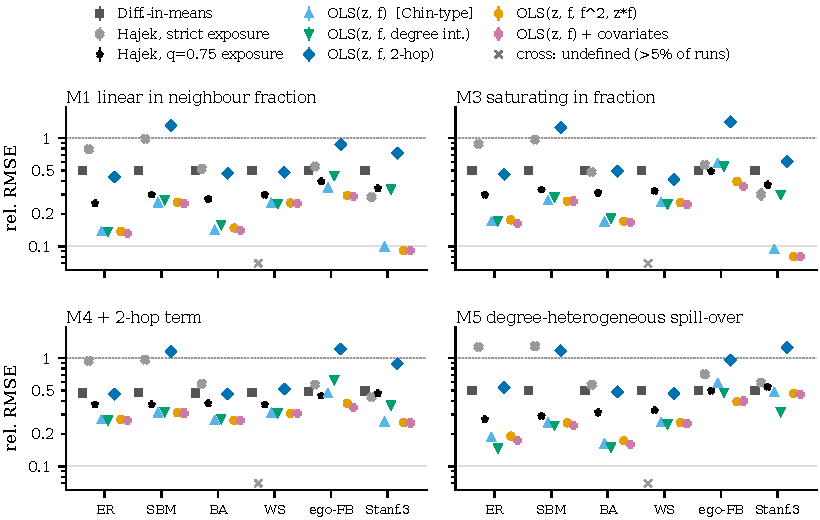
\includegraphics[width=0.99\linewidth]{fig1_headline.pdf}
\caption{Relative RMSE (RMSE$/|\gate|$, log scale, 95\% bootstrap CI) of each estimator on the 24 mechanism$\times$graph cells of the main grid under Bernoulli$(0.5)$, $\rho=1$. The difference in means has relative RMSE $\approx0.5$ everywhere because it recovers only the direct effect. Cells in which the strict H\'ajek estimator is undefined in more than 5\% of replicates are drawn as crosses. Other designs: Figures~\ref{fig:a1a}--\ref{fig:a1b}.}
\label{fig:headline}
\end{figure}
Figure~\ref{fig:headline} and Table~\ref{tab:failure} give the headline. Under Bernoulli$(0.5)$ with linear exposure (M1) the Chin-type OLS has median relative RMSE \MainOneOls{} across the six graphs against \MainDM{} for DM, and it is closer to the truth than DM in every graph of the main grid (Table~\ref{tab:failure}). Among the synthetic graphs, ER and BA (\MainOlsEr, \MainOlsBa) are easier than the SBM and Watts--Strogatz (\MainOlsSbm, \MainOlsWs); of the real graphs Stanford3 is easy (\MainStanOls) and ego-Facebook (\MainEgoOls) depends on the baseline draw (Fig.~\ref{fig:headline}; Sec.~\ref{sec:struct}). The strict H\'ajek estimator is no competitor under Bernoulli designs: it is undefined in a median of \HajekUndefBernLow{} of replicates at $p=0.1$, and at $p=0.5$ worse than OLS$(z,f)$ in every graph ($0.28$--$1.23$ against $0.10$--$0.34$). Adding a feature the mechanism does not need (the two-hop regressor under M1) is mainly a variance cost and is worse than DM on the SBM (\MainTwohopOneSbm), ego-Facebook (\MainTwohopOneEgo) and Stanford3 (\MainTwohopOneStan). The advantage is not uniform: under the saturating mechanism M3 at $p=0.1$ the Chin-type OLS has median relative RMSE \MainThreeBernLow{} and median relative bias \MainThreeBernLowBias{}, and it loses to DM on five of six graphs; only Stanford3, with its degree of 98, is better (Table~\ref{tab:failure}); two-hop interference (M4) gives a median relative bias of \MainFourBias{} at $p=0.5$, which a two-hop feature removes (\MainFourTwohopBias) at a variance price.

\begin{table}[t]
\centering\small
\caption{Main grid, median over six graphs [min, max] of relative RMSE of DM and of OLS$(z,f)$, median relative bias of OLS$(z,f)$, and the number of graphs on which OLS$(z,f)$ is better than / worse than / not significantly different from DM in paired MSE (95\% bootstrap CI of the MSE ratio, \texttt{results/contrasts.csv}).}
\label{tab:failure}
\begin{tabular}{@{}llccrc@{}}
\toprule
 & & \multicolumn{2}{c}{rel.\ RMSE, median [min, max]} & rel.\ bias & OLS better /\\
mech. & design & DM & OLS$(z,f)$ & OLS$(z,f)$ & worse / n.s.\ \\
\midrule
M1 & Bernoulli(0.5) & 0.50 [0.50, 0.50] & 0.19 [0.10, 0.34] & +0.00 & 6 / 0 / 0 \\
M1 & Bernoulli(0.1) & 0.50 [0.50, 0.51] & 0.31 [0.16, 0.57] & +0.00 & 5 / 1 / 0 \\
M1 & graph-cluster (p=0.5) & 0.27 [0.15, 0.37] & 0.18 [0.13, 0.25] & +0.00 & 4 / 1 / 1 \\
\addlinespace
M3 & Bernoulli(0.5) & 0.50 [0.50, 0.50] & 0.21 [0.09, 0.58] & -0.09 & 5 / 1 / 0 \\
M3 & Bernoulli(0.1) & 0.50 [0.50, 0.51] & 0.63 [0.30, 0.80] & +0.53 & 1 / 5 / 0 \\
M3 & graph-cluster (p=0.5) & 0.31 [0.18, 0.40] & 0.17 [0.16, 0.70] & -0.05 & 4 / 1 / 1 \\
\addlinespace
M4 & Bernoulli(0.5) & 0.48 [0.47, 0.49] & 0.29 [0.26, 0.47] & -0.22 & 5 / 0 / 1 \\
M4 & Bernoulli(0.1) & 0.48 [0.47, 0.50] & 0.38 [0.28, 0.63] & -0.21 & 5 / 1 / 0 \\
M4 & graph-cluster (p=0.5) & 0.33 [0.17, 0.40] & 0.22 [0.16, 0.59] & -0.06 & 3 / 2 / 1 \\
\addlinespace
M5 & Bernoulli(0.5) & 0.50 [0.50, 0.50] & 0.25 [0.16, 0.58] & -0.09 & 5 / 1 / 0 \\
M5 & Bernoulli(0.1) & 0.50 [0.50, 0.51] & 0.42 [0.23, 0.71] & -0.09 & 4 / 1 / 1 \\
M5 & graph-cluster (p=0.5) & 0.31 [0.17, 0.38] & 0.18 [0.16, 0.44] & -0.09 & 3 / 1 / 2 \\
\bottomrule
\end{tabular}

\end{table}

\subsection{RQ2: what determines the error?}
\paragraph{Variance dominates when the model is right, and is set by the design.}
Under correct specification the estimator is unbiased (|relative bias| $\le$ \EoneBiasMax{} for all $n$) and its SD falls as $n^{\EoneSlope}$ (fitted log--log slope; Fig.~\ref{fig:size}). Because DM has a constant bias of \EoneDMbias{} of the effect, OLS crosses it near $n=2{,}000$: at $n=500$ the regression is worse than DM (\EoneOLSA{} vs.\ \EoneDMA), at $n=8{,}000$ it is better (\EoneOLSC{} vs.\ \EoneDMC). The absolute SD of OLS is almost independent of the interference strength ($0.62$--$0.76$), so its error \emph{relative} to the effect $(1+\rho)$ falls with $\rho$ (Fig.~\ref{fig:gamma}); DM is much better with no interference ($\rho=0$: \EthreeDMZ{} vs.\ \EthreeOLSZ) and still better at $\rho=0.5$ (\EthreeDMH{} vs.\ \EthreeOLSH), and worse from $\rho=1$ (\EthreeDMO{} vs.\ \EthreeOLSO); at $\rho=4$ OLS has \EthreeOLSF{} against \EthreeDMF. Which graph quantities set the variance is predicted by P2: the SD grows with the (harmonic mean) degree, because the regressor $f$ then varies little across units and the coefficient of $f$ is weakly identified, and with the part of the baseline that is smooth over the graph. The predicted SD tracks the simulated one over \TheoryVarN{} graph draws (median ratio \TheoryVarMed, IQR \TheoryVarLo--\TheoryVarHi; Fig.~\ref{fig:theory}). Concretely, on the SBM the relative RMSE grows from \EtwoSbmLo{} at mean degree 5 to \EtwoSbmHi{} at 160, where DM would be better; on ER it grows more slowly (\EtwoErLo{} to \EtwoErHi, Fig.~\ref{fig:degree}). A community-level component of the baseline raises the error most: with $\sigma_c=0$ the relative RMSE is \EnineCzero{}, with $\sigma_c=3$ it is \EnineCthree{} (Fig.~\ref{fig:noise}), which is above DM's $0.5$.

\begin{figure}[t]
\centering
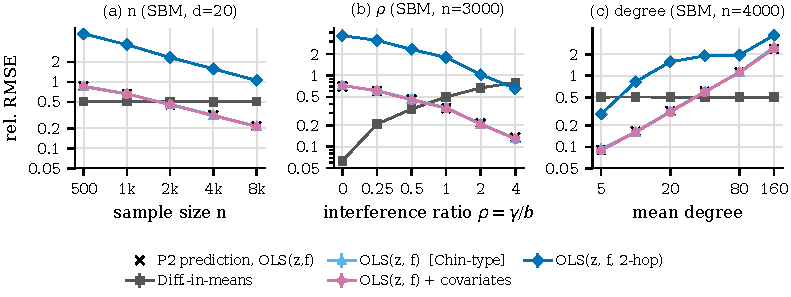
\includegraphics[width=0.96\linewidth]{figM_rmse_sweeps.pdf}
\caption{Relative RMSE of DM and OLS variants against (a) $n$ (SBM, mean degree 20), (b) the interference ratio $\rho$ ($n=3{,}000$) and (c) mean degree ($n=4{,}000$); 8 graph draws $\times$ 250 assignments per point. Crosses: closed-form P2 standard deviation of OLS$(z,f)$. Covariates change nothing visible; the two-hop regressor is worse except at $\rho=4$. Bias and SD panels, with the count-feature variants, are in Figs.~\ref{fig:sizeapp}--\ref{fig:gammaapp}.}
\label{fig:size}\label{fig:gamma}
\end{figure}

\paragraph{Bias comes from extrapolation and specification.}
The regression is fit where the exposure $f$ is concentrated near the design's $p$ and then evaluated at $f=0$ and $f=1$. P1 turns this into a computable asymptotic bias, $\beta_f^*-[g(1)-g(0)]$, which matches the noise-free population fits in \TheoryBiasN{} graph draws (correlation \TheoryBiasCorr, maximum absolute difference \TheoryBiasMaxDiff). Figure~\ref{fig:curv} shows what it implies: for each smooth response the bias vanishes at one value of $p$ and changes sign around it (for $f^{0.5}$ at degree 10 the relative bias is \EfourPowLo{} at $p=0.1$ and \EfourPowHi{} at $p=0.9$; for $f^2$ it is \EfourQuadMid{} at $p=0.5$ and \EfourQuadLo{}, \EfourQuadHi{} at $p=0.1,0.9$); for a threshold response at $f=0.5$ it is \EfourThrMidDten{} at $p=0.5$ and \EfourThrLoDten{}, \EfourThrHiDten{} at $p=0.1,0.9$. It is a population quantity, so more data do not reduce it, and higher degree does not either, since it concentrates $f$ around $p$: the threshold bias at $p=0.5$ grows from \EfourThrMidDten{} (degree 10) to \EfourThrMidDhund{} (degree 160). Whether a feature set can express the mechanism matters in the same way (Fig.~\ref{fig:spec}): adding a two-hop term to the signal gives a relative bias of \EsixTwohopBias{} for the Chin-type OLS on the SBM. The raw neighbour \emph{count} (scaled by mean degree) is confounded with degree and hence with the degree-correlated baseline: on ER with mean degree 60 its relative RMSE is \EsixCntErFrac{} when the truth is the fraction and \EsixCntEr{} when the truth is the count itself, and its relative bias is \EthreeCntZ{} even with no interference ($\rho=0$, Fig.~\ref{fig:gammaapp}). Controlling for log-degree and clustering removes this on ER (\EsixCntAdjErFrac{} and \EsixCntAdjEr), but on BA with fraction exposure the same adjusted regression has a relative bias of \EsixCntAdjBaBias{} (Fig.~\ref{fig:spec}). Heterogeneous spillovers that correlate with degree bias the estimator by P3 (M5 in Table~\ref{tab:failure}).
\begin{figure}[t]
\centering
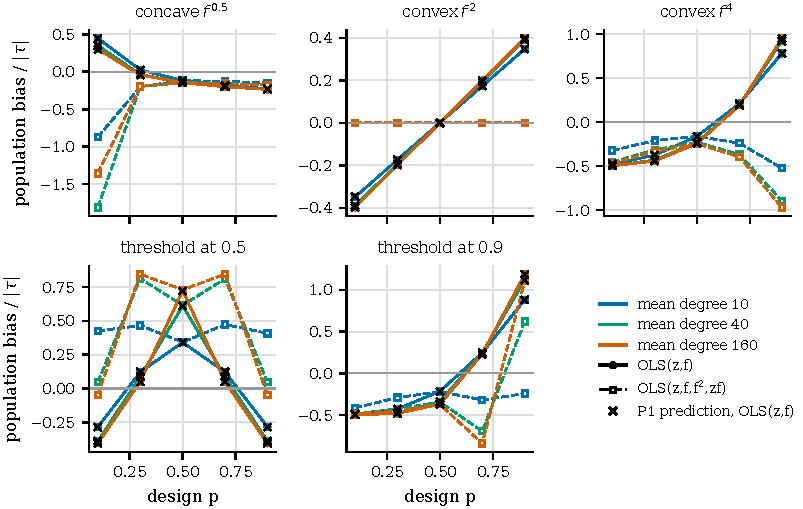
\includegraphics[width=0.97\linewidth]{fig8_curvature_population_bias.pdf}
\caption{Population (noise- and baseline-free) bias of OLS$(z,f)$ and of the quadratic OLS$(z,f,f^2,zf)$ relative to $|\gate|$, against the design $p$, for convex ($f^2$, $f^4$), concave ($f^{0.5}$) and threshold responses and mean degrees 10, 40, 160 (SBM, $n=3{,}000$). The estimand is exact; no sampling error enters. OLS$(z,f)$ is unbiased only at special $p$; the quadratic model removes the bias only when the truth is quadratic.}
\label{fig:curv}
\end{figure}

\paragraph{Flexible learners do not remove it.}
H2 predicted that tree ensembles, which do not extrapolate, would fail. The evidence is mixed (Fig.~\ref{fig:model}; fewer replicates: 4 graph draws $\times$ 80 assignments). Under linear exposure, ridge regression on rich features (relative RMSE \EsevenLinARidge{} at degree 10, \EsevenLinBRidge{} at degree 40) and a cubic OLS at degree 40 (\EsevenLinBCub) are far worse than OLS$(z,f)$ (\EsevenLinAOls, \EsevenLinBOls); boosting (\EsevenLinAGbm, \EsevenLinBGbm) is biased towards zero at degree 40 (relative bias \EsevenBiasLinBGbm). Under the threshold response OLS$(z,f)$ is biased (\EsevenBiasThrAOls{} and \EsevenBiasThrBOls{} at degrees 10 and 40), boosting is nearly unbiased (\EsevenBiasThrAGbm{}, \EsevenBiasThrBGbm) and has lower RMSE than OLS$(z,f)$ at degree 40 (\EsevenThrBGbm{} vs.\ \EsevenThrBOls) but not at degree 10 (\EsevenThrAGbm{} vs.\ \EsevenThrAOls); the cubic OLS is best at degree 10 (\EsevenThrACub) and worst at degree 40 (\EsevenThrBCub). No learner dominates; the bias--variance trade-off moves with the degree.
\begin{figure}[t]
\centering
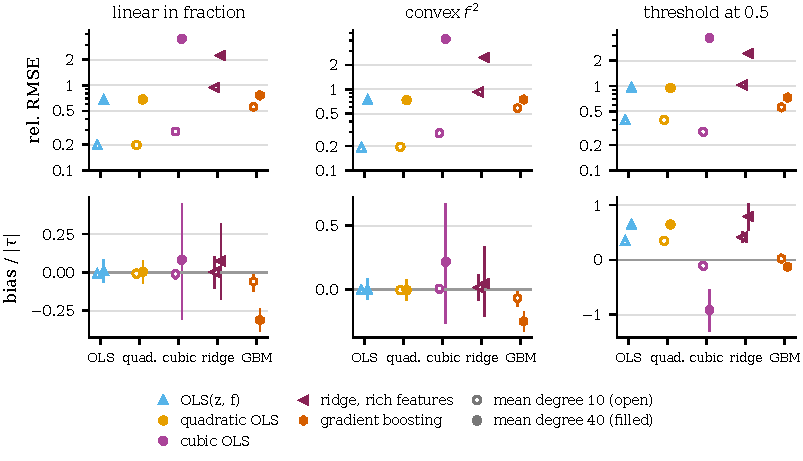
\includegraphics[width=0.97\linewidth]{fig15_model_class.pdf}
\caption{Model class (OLS, quadratic and cubic OLS, ridge on rich features, gradient boosting) under linear, convex and threshold exposure (SBM, $n=3{,}000$, $p=0.5$; open: mean degree 10, filled: 40). Relative RMSE and bias with bootstrap CIs; 4 graph draws $\times$ 80 assignments.}
\label{fig:model}
\end{figure}

\paragraph{A computable diagnostic works only for one family (negative result).}
H7 proposed that a data-computable exposure-support statistic, the distance (in SDs of the realised $f$) from the design's mean exposure to the farther of $f=0,1$, predicts the extrapolation error. Under Bernoulli designs it does for the saturating mechanism ($R^2=\HsevenSat$ in a log--log regression across cells) but not for power (\HsevenPow), threshold (\HsevenThresh), degree-heterogeneous (\HsevenHet) or two-hop (\HsevenBernTwohop) responses; pooled over all misspecified cells it explains $R^2=\HsevenPooled$ (\texttt{results/h7.csv}; Fig.~\ref{fig:h7} in the appendix shows the main grid). Within the ten cluster-randomised cells per mechanism the statistic is high for saturating (\HsevenClSat), two-hop (\HsevenClTwohop) and heterogeneous (\HsevenClHet) responses, but these are ten cells per mechanism that differ across graph families and not across $p$, so we do not weigh them against the Bernoulli result. We do not recommend the statistic as a general warning signal: it tells how far the extrapolation is, not whether the response is curved there.

\subsection{RQ3: where does it hold, where does it fail?}
\paragraph{Design.} Graph-cluster randomisation changes the conclusion: the median relative RMSE of DM falls from \MainDM{} to \MainDMClOne--\MainDMClFour{} across mechanisms (range $0.15$--$0.40$) because exposure is more often all-or-nothing, so the regression's advantage over DM under Bernoulli designs (\MainOneOls{} vs.\ \MainDM) largely disappears (Fig.~\ref{fig:design}); OLS is still better than DM in 14 of the 24 cluster-design graph--mechanism pairs (worse in 5, not distinguishable in 5; Table~\ref{tab:failure}), with OLS medians \MainOlsClThree--\MainOlsClFour{} against DM's. It also reduces extrapolation bias (M4: \MainFourBias{} $\to$ \MainFourBiasCl{} in Table~\ref{tab:failure}); for M3 the median OLS error under cluster randomisation (\MainOlsClThree) is close to that under the linear mechanism (\MainOlsClOne). A small $p$ is costly: variance rises as $1/\sqrt{p(1-p)}$ and nonlinear responses are extrapolated further (Table~\ref{tab:failure}, Bernoulli$(0.1)$ rows).

\paragraph{Network structure.}\label{sec:struct} OLS$(z,f)$ beats DM on \EfiveBetterN{} of ten graph families (relative RMSE \EfiveLo--\EfiveHi{} against DM's $0.5$) but not on ego-Facebook, where in this draw it is worse (\EfiveEgo; Fig.~\ref{fig:families}). The main grid and E5 use one draw of the synthetic baseline per real graph, and the same ego-Facebook specification gives a relative RMSE of \MainEgoOls{} in the main grid, \EelevenEgoZero{} in E11 and \EfiveEgo{} here, so we reran the 24 real-graph main cells with 8 independent baseline draws (60 assignments each). Under M1 and Bernoulli$(0.5)$ the relative RMSE of OLS$(z,f)$ on ego-Facebook has mean \RdEgoOneMean{} over the draws (range \RdEgoOneLo--\RdEgoOneHi, SD \RdEgoOneSd) against \RdEgoOneDM{} for DM, and on Stanford3 \RdStanOneMean{} (\RdStanOneLo--\RdStanOneHi). Over the four mechanisms at $p=0.5$ OLS beats DM in \RdStanWinsHalf{} of 32 draw--mechanism pairs on Stanford3 (\RdStanWinsTenth{} of 32 at $p=0.1$, \RdStanWinsCl{} under cluster randomisation) but in only \RdEgoWinsHalf{} of 32 on ego-Facebook (\RdEgoWinsTenth{} of 32 at $p=0.1$, \RdEgoWinsCl{} under cluster randomisation), with the saturating and degree-heterogeneous mechanisms the worst (\RdEgoThreeHalf{} and \RdEgoFiveHalf{} of 8). So Stanford3 favours regression robustly, whereas on ego-Facebook the answer depends on the baseline draw and DM is competitive; the count of families above is a single-draw count for ego-Facebook. Degree is the main structural driver (above); clustering and block structure matter through the baseline projection in P2 (at equal mean degree 20 and $n=4{,}000$ the relative RMSE is \EfiveEr{} on ER, \EfiveSbmMid{} on the SBM with $40\%$ of edges between blocks and \EfiveSbmLo{} with $2\%$; Fig.~\ref{fig:families}).

\paragraph{Graph errors.} Dropping and re-adding a share of edges when building the features biases the estimate towards zero, monotonically in the error rate, by $\EelevenSbmBias|\gate|$ at $50\%$ on the SBM and $\EelevenEgoBias|\gate|$ on ego-Facebook (Fig.~\ref{fig:grapherr}). At $\rho=1$ the relative RMSE rises from \EelevenSbmZero{} to \EelevenSbmGOne{} on the SBM (DM: \EelevenSbmGOneDM) and stays below DM, whereas on ego-Facebook it is already \EelevenEgoZero{} without errors and \EelevenEgoGOne{} at $50\%$ (about DM's level). With weak interference ($\rho=0.25$) the regression with an error-free graph already has relative RMSE \EelevenWeakOls{} against \EelevenWeakDM{} for DM, so DM wins at every error rate on both graphs.

\paragraph{Inference.} In the correctly specified linear mechanism the cluster-robust 95\% interval covers between \CovClMin{} and \CovClMax{} across graph families and sizes, below the nominal $95\%$ although the bias is negligible: on the SBM it improves with $n$ (\CovClSbmSmall{} at $n=1{,}000$ to \CovClSbmN{} at $4{,}000$), on BA it worsens (\CovClBaA{} to \CovClBaB). The interval that treats units as independent covers only \CovHcSbmLoA{} at $n=1{,}000$ and \CovHcSbmLoB{} at $4{,}000$ when baselines are community-structured and mixing is weak (\CovHcSbmMix{} and \CovHcSbmMixB{} for strong mixing), so its under-coverage grows with $n$; it covers $0.87$--$0.92$ on ER and BA (Fig.~\ref{fig:cover}). On the main grid coverage collapses once $|\text{bias}|/\mathrm{SD}>1$ (Fig.~\ref{fig:cov-bias}), as expected for an interval centred on a biased estimate. How coverage changes with $n$ when the model is misspecified (the second part of H6) was not tested.
\begin{figure}[t]
\centering
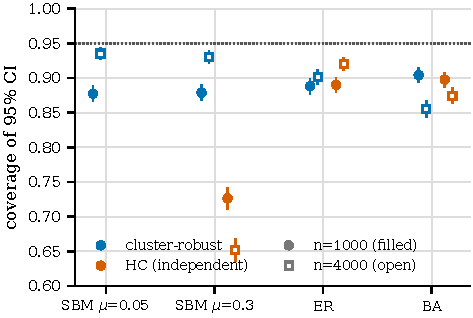
\includegraphics[width=0.57\linewidth]{fig13_coverage_n.pdf}
\caption{Coverage of the nominal 95\% interval for OLS$(z,f)$, cluster-robust versus independent-units standard errors, $n=1{,}000$ (filled) and $4{,}000$ (open), correct linear mechanism, 10 graph draws $\times$ 300 assignments.}
\label{fig:cover}
\end{figure}


\section{Discussion and Limitations}
\label{sec:discussion}
\paragraph{What the evidence says.}
Against the seven hypotheses we pre-specified (Table~\ref{tab:hyp}, Appendix), H1, H3 and H5 are supported, H2, H4 and H6 partly, and H7 not as a general law.
Regression adjustment for the GATE is a bias--variance bargain whose terms are set by the design and the graph, not by the sample size alone. When the exposure model is right it is the most accurate of the estimators we compared once $n$ and the interference are large enough (in the default SBM setting, $n\gtrsim2{,}000$ and interference at least as strong as the direct effect; the break-even moves with degree and confounding); under Bernoulli$(0.5)$ its median relative RMSE over the six main-grid graphs is then \MainOneOls{} (DM: \MainDM). It is not a free lunch: its variance grows with degree and with community-level baseline confounding, and a difference in means is better with weak interference, small $n$, or after cluster randomisation. When the exposure model is wrong, the error is a bias that more data do not remove; we can compute its first-order size in the linear family (P1) and observe it for nonlinear, two-hop, degree-heterogeneous and miswired responses.
\paragraph{Practical reading.} (i) Fit the simplest exposure model, but check the design's exposure support: bias is largest where $f$ is far from the design's mean exposure. (ii) Prefer balanced designs; at $p=0.1$ nonlinear bias and variance both grow. (iii) Do not rely on high-capacity learners to escape misspecification. (iv) Treat nominal $95\%$ intervals, cluster-robust ones included, as optimistic. These are readings of simulations.
\paragraph{Limitations.}
\emph{Synthetic outcomes.} The graphs are real or generated, but every outcome is simulated from mechanisms we chose; we did not test the estimators on any experiment with real outcomes, and our mechanisms (linear, saturating, power, threshold, two-hop, degree-heterogeneous) are a small family. The relative scale (e.g.\ DM at $0.5$) is a function of the ratio $\rho$ we chose. \emph{Replication.} Synthetic cells use 5--8 graph draws; each real graph is one graph, and its baseline draw, which the bootstrap does not cover, matters (Sec.~\ref{sec:struct}). Sweeps vary one factor at a time. The model-class comparison (Fig.~\ref{fig:model}) uses 4 graph draws $\times$ 80 assignments, and a ridge/boosting evaluation on the full main grid was not completed (an attempt was stopped; Appendix~\ref{app:setup}). \emph{Analytics.} P1--P3 are first-order large-$n$ arguments for the linear-exposure family, checked numerically, not proved, and do not cover boosted or cubic fits. \emph{Inference.} Louvain communities are both the cluster design and, in some cells, the variance clusters, which favours the cluster-robust interval; we studied no corrections. \emph{Not done.} Multi-$p$ and staggered designs (H4), the dependence of coverage on $n$ under misspecification (H6), unknown-interference-radius selection, and optimal-design recommendations. The H7 diagnostic did not generalise, so we offer no data-driven warning signal.


\bibliographystyle{plainnat}
\bibliography{references}

\appendix
\section{Setup and reproduction}
\label{app:setup}
Table~\ref{tab:setup} summarises the simulation grid. All code, the data-acquisition steps with checksums, seeds, commands and the figure/table-to-script map are in the supplementary material (\texttt{code/README.md}, \texttt{figures/README.md}); every number quoted in the text is generated into \texttt{paper/numbers.tex} by \texttt{paper/scripts/make\_numbers.py} from \texttt{results/}. Base seed $20261102$. The 24 real-graph cells of the main grid were rerun with 8 independent baseline draws $\times$ 60 assignments (experiment \texttt{MAIN\_realdraws}, Sec.~\ref{sec:struct}). No material excluded by the task was consulted.
\paragraph{Estimator details.} All OLS variants use ordinary least squares on the listed features plus an intercept (``covariates'' are standardised log-degree and local clustering coefficient). The ridge regression uses the nine features $z,f,(W^2\bz),f^2,zf,\ell,f\ell,z\ell,c$ and the scaled neighbour count ($\ell$ standardised log-degree, $c$ clustering), standardised, with the penalty chosen by leave-one-out cross-validation over $13$ values in $[10^{-3},10^3]$. Gradient boosting is scikit-learn's \texttt{HistGradientBoostingRegressor} (200 iterations, learning rate $0.1$, at most 15 leaves, fixed seed) on $(z,f,W^2\bz,\ell,c)$. Neither learner is tuned per cell. DM is the treated--control difference of means; the strict H\'ajek estimator contrasts treated units whose neighbours are all treated with control units whose neighbours are all control, weighted by inverse design probabilities (undefined if either group is empty); the $q=0.75$ version relaxes ``all'' to at least $75\%$ of neighbours and is implemented for Bernoulli designs only.
\paragraph{Compute.} All runs are CPU-only, in containers limited to 2 CPUs and 4\,GB on a shared host (Xeon Gold 6230, load about 30), so the wall times below are upper bounds for an idle machine; one cell runs per process on 2 processes. Measured wall time: the main grid with the validity cells (76 cells) 21 min; the second-seed rerun (48 cells) 18 min; sweeps E1--E3, E5, E6, E8--E10 together 95 min; E4 (90 cells) 53 min; E11 about 2.5 min; analytic checks 38 min; export 32\,s. The model-class experiment E7 (ridge and boosting) took 21 h because the learners oversubscribed the host's threads; with threads limited, a pilot needs about 0.4\,s per replicate. A first attempt at the same learners on the full main grid was stopped after 38 h and is not reported. Peak memory is about 1.5\,GB per process for Stanford3 and 3.5\,GB for the export; per-group memory was not otherwise measured. The experiment table and the commands are in \texttt{code/README.md}; the code regenerates the delivered cell specifications, and a check script re-runs a cell and compares it with the stored replicates (identical for the cells we checked, including the main grid).
\begin{table}[H]
\centering\small
\caption{Setup of the main grid.}
\label{tab:setup}
\begin{tabular}{@{}lp{9.2cm}@{}}
\toprule
\multicolumn{2}{@{}l}{\textbf{Graphs} (size $n$, mean degree $\bar d$, replicates per cell)} \\
\hspace{1em}ER & $n=2{,}000$, $\bar d=10.0$, 5 graph draw(s) $\times$ 100 assignments \\
\hspace{1em}SBM & $n=2{,}000$, $\bar d=10.0$, 5 graph draw(s) $\times$ 100 assignments \\
\hspace{1em}BA & $n=2{,}000$, $\bar d=10.0$, 5 graph draw(s) $\times$ 100 assignments \\
\hspace{1em}WS & $n=2{,}000$, $\bar d=10.0$, 5 graph draw(s) $\times$ 100 assignments \\
\hspace{1em}ego-FB & $n=4{,}039$, $\bar d=43.7$, 1 graph draw(s) $\times$ 500 assignments \\
\hspace{1em}Stanford3 & $n=11{,}586$, $\bar d=98.1$, 1 graph draw(s) $\times$ 500 assignments \\
\midrule
\textbf{Mechanisms} & M1 linear in neighbour fraction $f_i$; M3 saturating $g(f_i)$; M4 = M1 + 2-hop term; M5 = M1 with degree-dependent spill-over. The GATE $\tau$ is computed exactly from $m(\mathbf 1)-m(\mathbf 0)$ (no rescaling); it equals $2$ in all four mechanisms (direct effect $1$, total spill-over $1$). \\
\textbf{Designs} & Bernoulli($0.5$), Bernoulli($0.1$), graph-cluster randomisation (Louvain, $p=0.5$). \\
\textbf{Estimators} & difference-in-means; Hajek exposure (strict and $q{=}0.75$); OLS on $(z,f)$, $(z,f,\text{degree int.})$, $(z,f,\text{2-hop})$, $(z,f,f^2,zf)$, $(z,f)$ + covariates. \\
\textbf{Metrics} & bias, SD, RMSE, RMSE$/|\tau|$ with bootstrap CIs over replicates; coverage of a cluster-robust 95\% interval. \\
\bottomrule
\end{tabular}

\end{table}

\section{Additional results}
\label{app:extra}
\paragraph{Hypotheses and verdicts.}
Table~\ref{tab:hyp} states each pre-specified hypothesis, the verdict from the evidence above, and its scope.
\begin{table}[H]
\centering\small
\caption{Pre-specified hypotheses and verdicts. ``Scope'': what was varied.}
\label{tab:hyp}
\begin{tabular}{@{}p{0.04\linewidth}p{0.36\linewidth}p{0.5\linewidth}@{}}
\toprule
 & Hypothesis (short) & Verdict (evidence) \\
\midrule
H1 & Correct spec.: unbiased, $n^{-1/2}$, beats DM more as $\rho$ grows & \textbf{Supported}, with a caveat: DM wins for small $n$ or $\rho$ (Fig.~\ref{fig:size}) \\
H2 & Misspecification bias persists with $n$; flexible learners do not fix it & \textbf{Partly supported}: bias is $n$-independent (P1, Fig.~\ref{fig:curv}); learners trade bias for variance, boosting helps under a threshold (Fig.~\ref{fig:model}) \\
H3 & Degree and clustering change the error; cluster designs help & \textbf{Supported}: degree sets the variance (P2); cluster designs reduce bias and DM's error; the extra variance expected from fewer independent units was not visible in the median error (Table~\ref{tab:failure}) \\
H4 & Balanced $p$ better than small $p$; multi-$p$ design helps & \textbf{Supported for} $p=0.5$ vs.\ $0.1$; multi-$p$/staggered designs \textbf{not tested} \\
H5 & Graph errors degrade accuracy monotonically & \textbf{Supported for bias} (towards zero, monotone in the error rate, Fig.~\ref{fig:grapherr}); RMSE is not monotone on ego-Facebook, and at weak interference DM wins even without error \\
H6 & Intervals under-cover when bias matters, worse with $n$ & \textbf{Partly}: under-coverage at $\approx0$ bias; the independent-units interval worsens with $n$ in community-structured graphs, the cluster-robust one improves on SBM but not on BA; collapse when $|$bias$|$/SD $>1$; the $n$-trend under misspecification \textbf{not tested} \\
H7 & A computable support statistic predicts the extrapolation error & \textbf{Not supported in general} ($R^2$ \HsevenPooled{} pooled; high only for the saturating family) \\
\bottomrule
\end{tabular}
\end{table}
\paragraph{Paired contrasts over all sweeps (Table~\ref{tab:contrasts}).}
For every experiment, each cell of the first-named estimator is compared with the second on the same draws and assignments; entries count cells where its MSE is smaller / not distinguishable / larger (95\% paired bootstrap intervals). OLS beats DM in most main-grid cells (50 smaller, 15 larger of 72) but loses in 64 of 90 curvature cells (E4); the two-hop regressor is worse than OLS$(z,f)$ in every main-grid cell, and OLS$(z,f)$ is never better than OLS with covariates in the main grid (worse in 32 of 72 cells).
\begin{table}[H]
\centering\scriptsize
\caption{Paired MSE contrasts (smaller / n.s. / larger) of the first estimator against the second, per experiment.}
\label{tab:contrasts}
\begin{tabular}{@{}lccccccc@{}}
\toprule
 & \shortstack{OLS\\vs DM} & \shortstack{OLS vs\\Hajek} & \shortstack{OLS vs\\quadr.} & \shortstack{OLS vs\\OLS$+$cov.} & \shortstack{2-hop\\vs OLS} & \shortstack{GBM\\vs OLS} & \shortstack{ridge\\vs OLS} \\
\midrule
main grid & 50/7/15 & 31/1/2 & 38/24/10 & 0/40/32 & 0/0/72 & -- & -- \\
main grid, seed 2 & 38/6/4 & 17/0/0 & 27/20/1 & 0/36/12 & 0/1/47 & -- & -- \\
E1 size $n$ & 3/0/2 & -- & 1/4/0 & 0/3/2 & 0/0/5 & -- & -- \\
E2 degree & 9/0/3 & -- & 7/5/0 & 0/1/11 & 0/0/12 & -- & -- \\
E3 $\rho$ & 3/0/3 & -- & 1/5/0 & 0/3/3 & 0/0/6 & -- & -- \\
E4 curvature $\times p$ & 24/2/64 & 33/2/1 & 78/12/0 & 1/70/19 & -- & -- & -- \\
E5 graph families & 9/0/1 & -- & 4/4/2 & 0/3/7 & 0/0/10 & -- & -- \\
E6 specification & 15/0/0 & -- & 11/4/0 & 0/4/11 & 0/0/15 & -- & -- \\
E7 model class & -- & -- & 1/5/0 & -- & -- & 1/1/4 & 0/0/6 \\
E8 design & 10/8/6 & -- & 15/9/0 & 1/18/5 & -- & -- & -- \\
E9 noise & 5/1/3 & -- & 3/6/0 & 0/4/5 & 0/0/9 & -- & -- \\
E10 coverage & -- & -- & -- & 0/4/12 & -- & -- & -- \\
E11 graph error & 7/5/12 & -- & 1/18/5 & 0/11/13 & -- & -- & -- \\
\bottomrule
\end{tabular}

\end{table}


\paragraph{Other designs (Fig.~\ref{fig:a1a}, \ref{fig:a1b}).} The headline figure for Bernoulli$(0.1)$ and cluster randomisation. At $p=0.1$ the strict H\'ajek estimator is undefined in almost all replicates (\HajekUndefBernLow); at $p=0.5$ in \HajekUndefBernHalf.
\begin{figure}[H]\centering
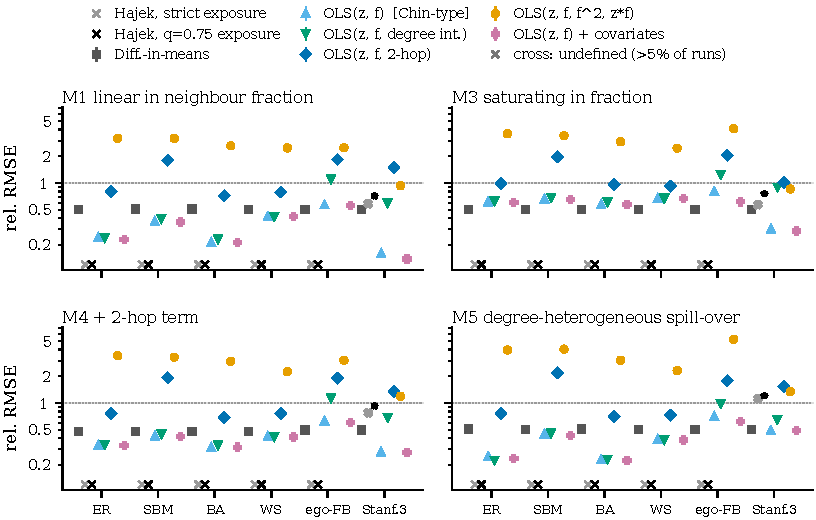
\includegraphics[width=0.99\linewidth]{figA1_headline_bern0.1.pdf}
\caption{As Fig.~\ref{fig:headline}, Bernoulli$(0.1)$.}\label{fig:a1a}
\end{figure}
\begin{figure}[H]\centering
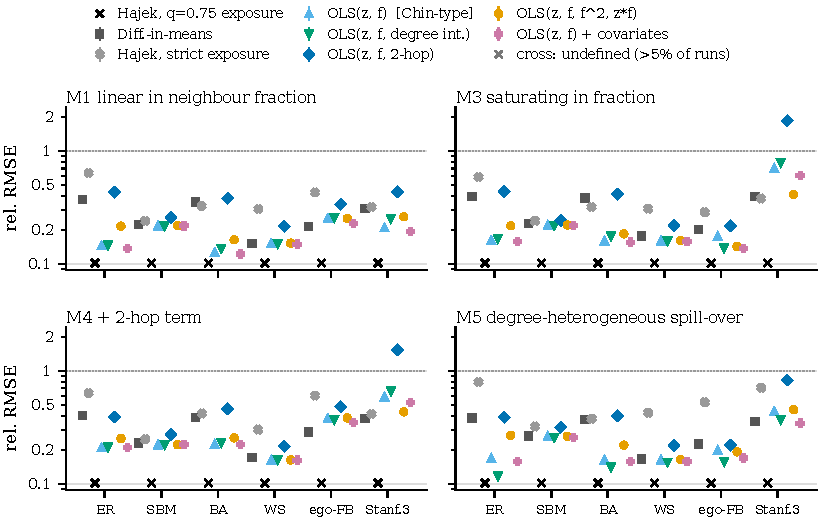
\includegraphics[width=0.99\linewidth]{figA1_headline_cluster0.5.pdf}
\caption{As Fig.~\ref{fig:headline}, graph-cluster randomisation ($p=0.5$).}\label{fig:a1b}
\end{figure}

\paragraph{Seed replication (Fig.~\ref{fig:seed}).}\label{app:seed} A second, independent seed set for the 48 synthetic main-grid cells reproduces the relative RMSE of every estimator.
\begin{figure}[H]\centering
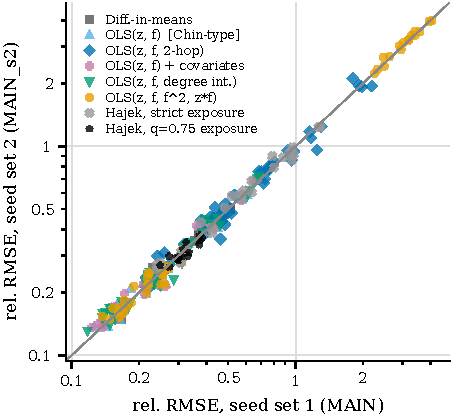
\includegraphics[width=0.55\linewidth]{figA2_seed_replication.pdf}
\caption{Relative RMSE under the first versus the second seed set, synthetic main-grid cells.}\label{fig:seed}
\end{figure}

\paragraph{Bias versus variance and coverage on the main grid (Figs.~\ref{fig:biassd}, \ref{fig:cov-bias}).}
\begin{figure}[H]\centering
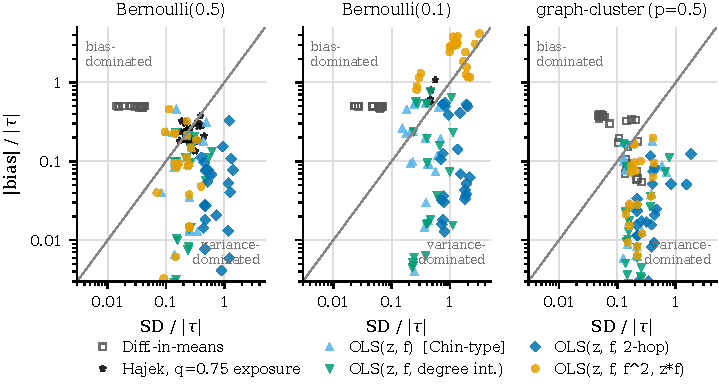
\includegraphics[width=0.87\linewidth]{fig2_bias_sd.pdf}
\caption{$|$Bias$|/|\gate|$ against SD$/|\gate|$ of each estimator, one point per main-grid cell, by design; the diagonal separates bias- from variance-dominated error.}\label{fig:biassd}
\end{figure}
\begin{figure}[H]\centering
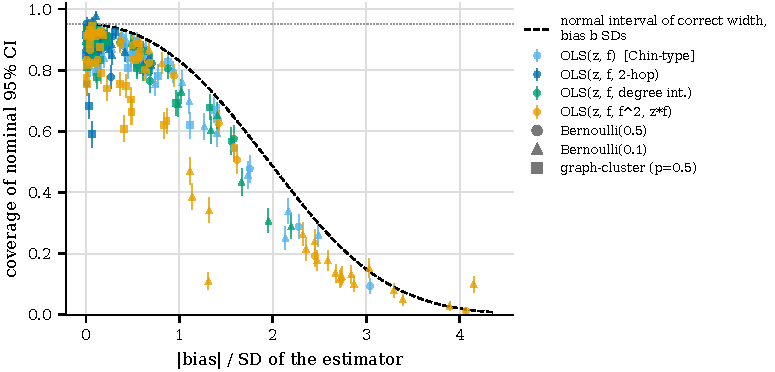
\includegraphics[width=0.94\linewidth]{fig4_coverage.pdf}
\caption{Coverage of the nominal 95\% interval against $|\text{bias}|/\mathrm{SD}$, main grid.}\label{fig:cov-bias}
\end{figure}


\paragraph{Diagnostic, design and graph errors (Figs.~\ref{fig:h7}, \ref{fig:design}, \ref{fig:grapherr}).}
\begin{figure}[H]
\centering
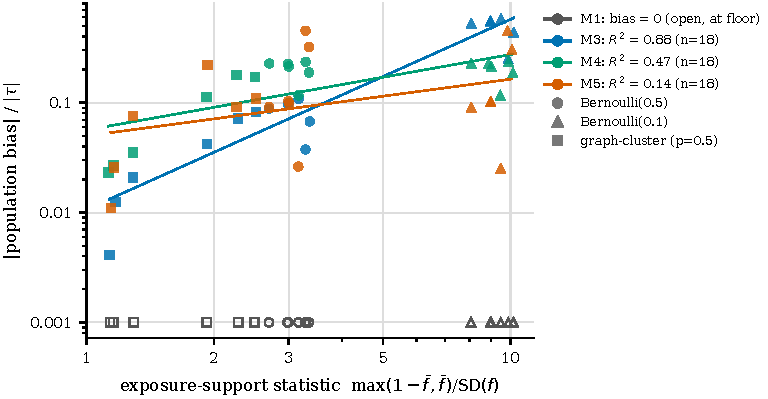
\includegraphics[width=0.93\linewidth]{fig3_h7_diagnostic.pdf}
\caption{Exposure-support statistic against the absolute population bias of OLS$(z,f)$ on the main grid, one point per cell, per-mechanism log--log regression; cells with no bias (M1) are drawn open at the floor.}
\label{fig:h7}
\end{figure}
\begin{figure}[H]
\centering
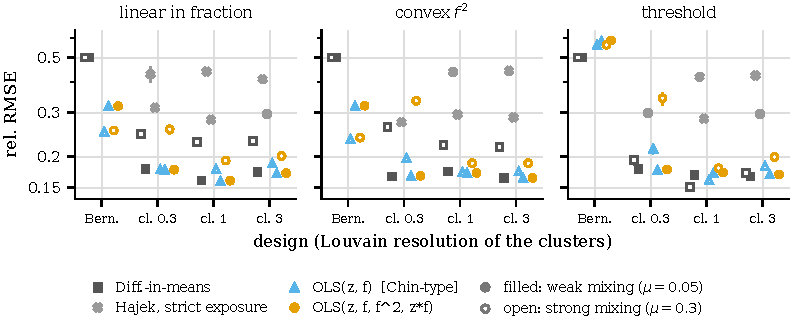
\includegraphics[width=0.96\linewidth]{fig12_design.pdf}
\caption{Bernoulli versus graph-cluster randomisation at three Louvain resolutions, weak (filled) and strong (open) mixing between blocks, for linear, convex and threshold exposure (SBM, $n=4{,}000$, mean degree 20).}
\label{fig:design}
\end{figure}
\begin{figure}[H]
\centering
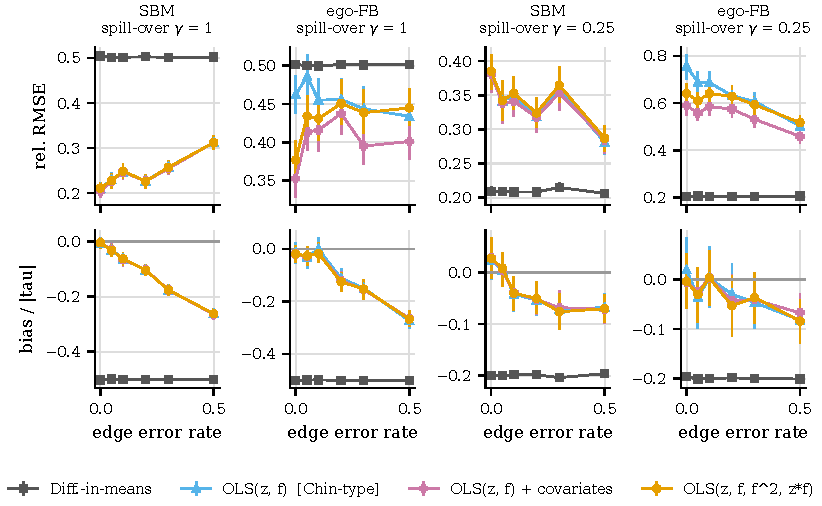
\includegraphics[width=1\linewidth]{fig5_graph_error.pdf}
\caption{Error against the share of edges dropped and re-added in the graph used to build $f$ (8 perturbation draws on the SBM, 12 on ego-Facebook), strong ($\rho=1$) and weak ($\rho=0.25$) interference.}
\label{fig:grapherr}
\end{figure}

\paragraph{Degree and noise (Figs.~\ref{fig:degree}, \ref{fig:noise}).}
\begin{figure}[H]\centering
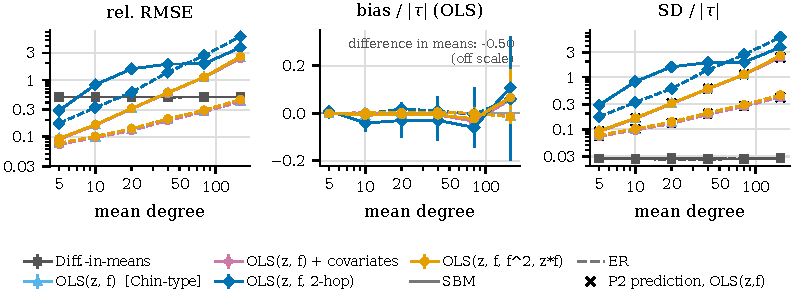
\includegraphics[width=0.96\linewidth]{fig10_degree.pdf}
\caption{Relative RMSE, relative bias and relative SD against mean degree for the Chin-type OLS$(z,f)$, its degree-interaction and quadratic variants and DM, on SBM (solid) and ER (dashed) graphs.}\label{fig:degree}
\end{figure}
\begin{figure}[H]\centering
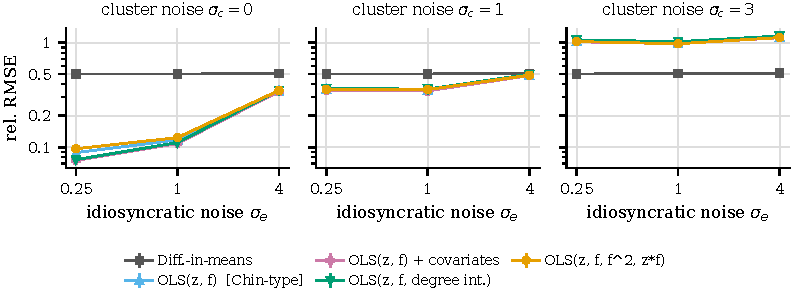
\includegraphics[width=0.96\linewidth]{fig16_noise.pdf}
\caption{Relative RMSE against the idiosyncratic noise SD $\sigma_e$ for community-level baseline SD $\sigma_c=0,1,3$ (SBM; DM grey).}\label{fig:noise}
\end{figure}

\paragraph{Bias and SD against $n$ and $\rho$ (Figs.~\ref{fig:sizeapp}, \ref{fig:gammaapp}).}
\begin{figure}[H]\centering
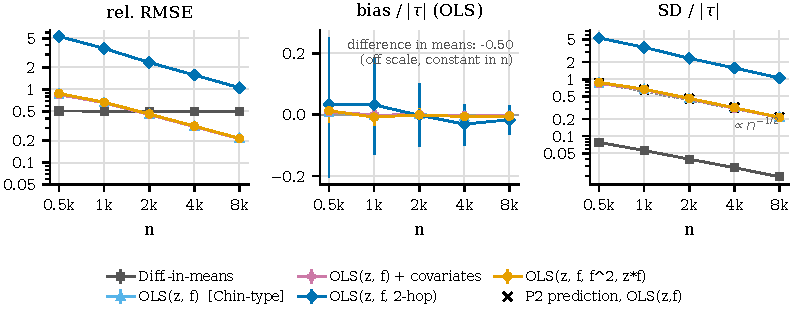
\includegraphics[width=0.96\linewidth]{fig6_size.pdf}
\caption{Bias, SD and relative RMSE against $n$ for the correctly specified linear mechanism (SBM, mean degree 20); the SD of OLS follows the $n^{-1/2}$ reference and the P2 prediction.}\label{fig:sizeapp}
\end{figure}
\begin{figure}[H]\centering
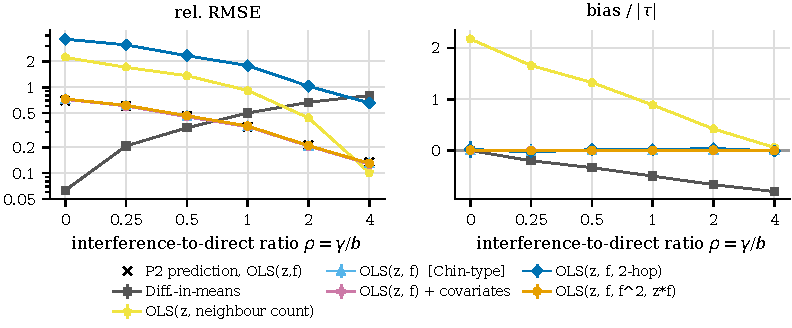
\includegraphics[width=0.96\linewidth]{fig7_gamma.pdf}
\caption{The same against the interference ratio $\rho$ ($n=3{,}000$). OLS on the raw neighbour count is strongly biased, most at $\rho=0$.}\label{fig:gammaapp}
\end{figure}

\paragraph{Feature set versus form of interference (Figs.~\ref{fig:spec}, \ref{fig:specbias}).}
\begin{figure}[H]\centering
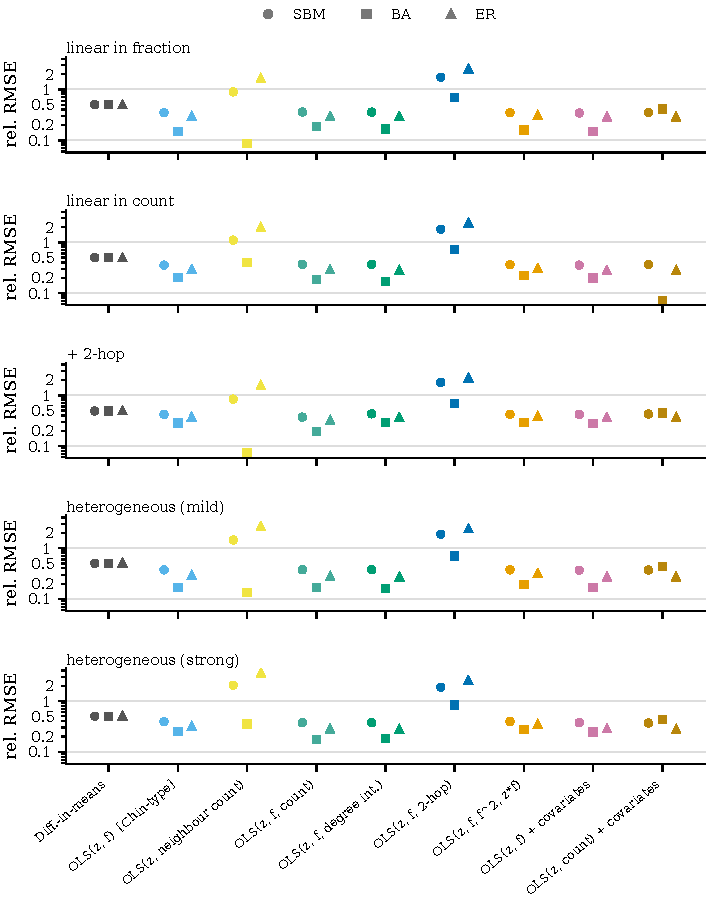
\includegraphics[width=0.86\linewidth]{fig11_specification.pdf}
\caption{Error of feature sets (rows) for different true exposure forms (linear fraction, linear count, two-hop, degree-heterogeneous) on ER, SBM and BA.}\label{fig:spec}
\end{figure}
\begin{figure}[H]\centering
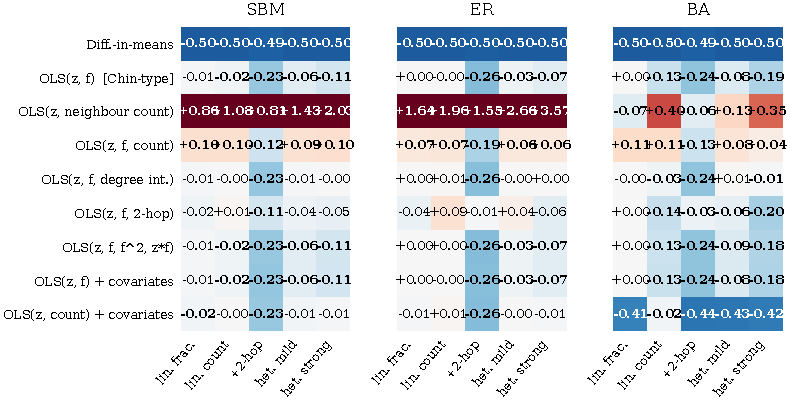
\includegraphics[width=0.96\linewidth]{fig11b_specification_bias.pdf}
\caption{Signed relative bias of the feature sets for each true exposure form (heat map; bold: interval excludes zero). OLS$(z,f)$ is within $\pm0.02$ on SBM and ER for the linear forms and about $-0.25$ under an omitted two-hop term; the degree interaction removes the heterogeneity bias but not the two-hop bias.}\label{fig:specbias}
\end{figure}

\paragraph{Graph families (Fig.~\ref{fig:families}) and observed error against $p$.}
\begin{figure}[H]\centering
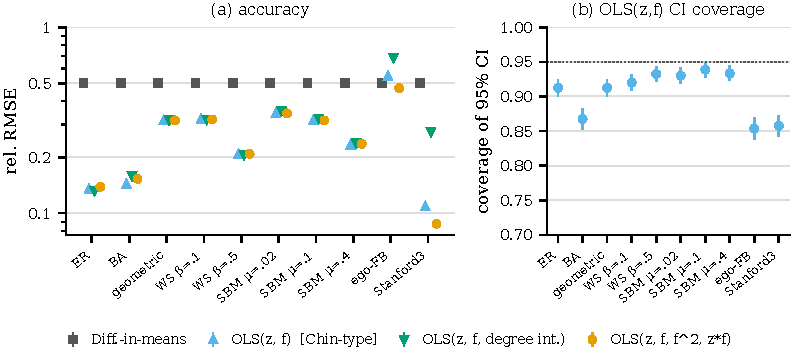
\includegraphics[width=0.96\linewidth]{fig14_graph_families.pdf}
\caption{Ten graph families (synthetic at $n=4{,}000$, mean degree 20, and the two Facebook graphs): (a) relative RMSE of DM and of OLS variants; (b) coverage of the 95\% interval for OLS$(z,f)$.}\label{fig:families}
\end{figure}
\begin{figure}[H]\centering
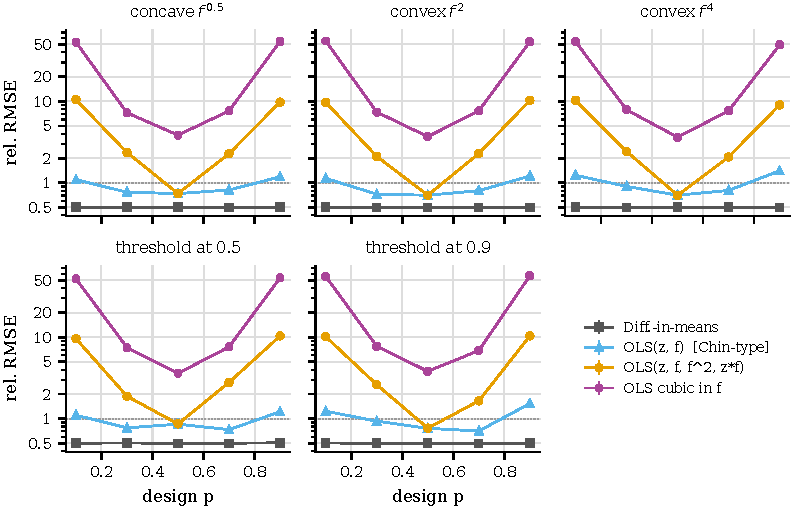
\includegraphics[width=0.96\linewidth]{fig9_curvature_rmse.pdf}
\caption{Observed relative RMSE against the design $p$ for the responses of Fig.~\ref{fig:curv} (degree 40); the quadratic model pays in variance what it gains in bias.}\label{fig:curvobs}
\end{figure}
\begin{figure}[H]\centering
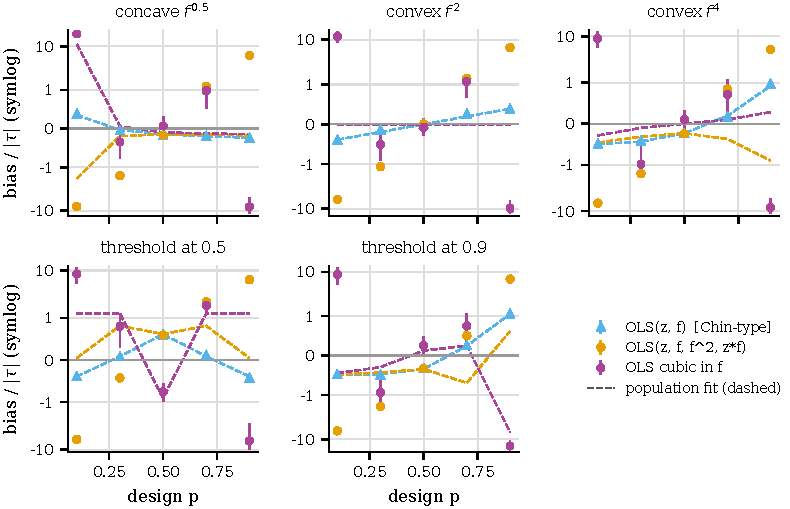
\includegraphics[width=0.96\linewidth]{fig9b_curvature_bias_observed.pdf}
\caption{Observed against population-fit bias (degree 40). For OLS$(z,f)$ the two agree; for the quadratic and cubic models the observed bias is far larger at $p=0.1,0.9$, i.e.\ they err by more than their approximation error (we did not test the cause).}\label{fig:curvbiasobs}
\end{figure}

\paragraph{Theory checks (Fig.~\ref{fig:theory}).}
\begin{figure}[H]\centering
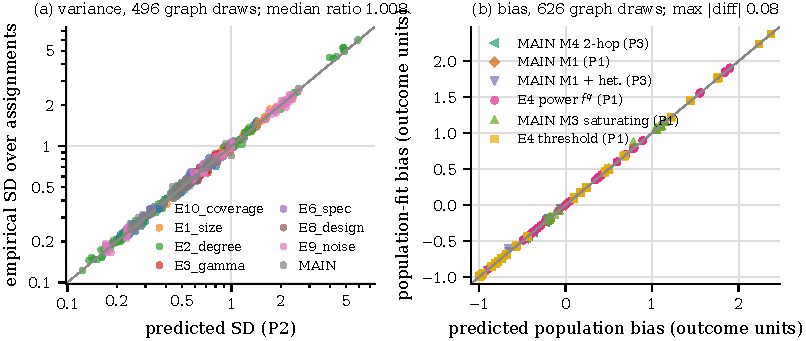
\includegraphics[width=0.98\linewidth]{fig17_theory_check.pdf}
\caption{(a) Predicted (P2) against empirical SD of OLS$(z,f)$ over \TheoryVarN{} graph draws from several experiments; (b) predicted (P1/P3) against noise-free population bias over \TheoryBiasN{} draws; both relative to $|\gate|$, diagonal is exact agreement.}\label{fig:theory}
\end{figure}


\clearpage
\section*{NeurIPS Paper Checklist}




\begin{enumerate}

\item {\bf Claims}
    \item[] Question: Do the main claims made in the abstract and introduction accurately reflect the paper's contributions and scope?
    \item[] Answer: \answerYes{}
    \item[] Justification: The abstract and Section~1 state the scope (simulated outcomes on six graphs, four mechanisms, three designs) and every claim is backed by Section~\ref{sec:experiments} and the appendix.
    \item[] Guidelines:
    \begin{itemize}
        \item The answer \answerNA{} means that the abstract and introduction do not include the claims made in the paper.
        \item The abstract and/or introduction should clearly state the claims made, including the contributions made in the paper and important assumptions and limitations. A \answerNo{} or \answerNA{} answer to this question will not be perceived well by the reviewers. 
        \item The claims made should match theoretical and experimental results, and reflect how much the results can be expected to generalize to other settings. 
        \item It is fine to include aspirational goals as motivation as long as it is clear that these goals are not attained by the paper. 
    \end{itemize}

\item {\bf Limitations}
    \item[] Question: Does the paper discuss the limitations of the work performed by the authors?
    \item[] Answer: \answerYes{}
    \item[] Justification: Section~\ref{sec:discussion} (Limitations) lists synthetic outcomes, the small mechanism family, replicate counts, first-order theory, inference and what was not run.
    \item[] Guidelines:
    \begin{itemize}
        \item The answer \answerNA{} means that the paper has no limitation while the answer \answerNo{} means that the paper has limitations, but those are not discussed in the paper. 
        \item The authors are encouraged to create a separate ``Limitations'' section in their paper.
        \item The paper should point out any strong assumptions and how robust the results are to violations of these assumptions (e.g., independence assumptions, noiseless settings, model well-specification, asymptotic approximations only holding locally). The authors should reflect on how these assumptions might be violated in practice and what the implications would be.
        \item The authors should reflect on the scope of the claims made, e.g., if the approach was only tested on a few datasets or with a few runs. In general, empirical results often depend on implicit assumptions, which should be articulated.
        \item The authors should reflect on the factors that influence the performance of the approach. For example, a facial recognition algorithm may perform poorly when image resolution is low or images are taken in low lighting. Or a speech-to-text system might not be used reliably to provide closed captions for online lectures because it fails to handle technical jargon.
        \item The authors should discuss the computational efficiency of the proposed algorithms and how they scale with dataset size.
        \item If applicable, the authors should discuss possible limitations of their approach to address problems of privacy and fairness.
        \item While the authors might fear that complete honesty about limitations might be used by reviewers as grounds for rejection, a worse outcome might be that reviewers discover limitations that aren't acknowledged in the paper. The authors should use their best judgment and recognize that individual actions in favor of transparency play an important role in developing norms that preserve the integrity of the community. Reviewers will be specifically instructed to not penalize honesty concerning limitations.
    \end{itemize}

\item {\bf Theory assumptions and proofs}
    \item[] Question: For each theoretical result, does the paper provide the full set of assumptions and a complete (and correct) proof?
    \item[] Answer: \answerNA{}
    \item[] Justification: The paper has no theorems; P1--P3 are first-order large-$n$ derivations (supplementary \texttt{code/docs/THEORY.md}) that we check numerically in Section~\ref{sec:experiments} and Fig.~\ref{fig:theory}, and we say they are not proofs.
    \item[] Guidelines:
    \begin{itemize}
        \item The answer \answerNA{} means that the paper does not include theoretical results. 
        \item All the theorems, formulas, and proofs in the paper should be numbered and cross-referenced.
        \item All assumptions should be clearly stated or referenced in the statement of any theorems.
        \item The proofs can either appear in the main paper or the supplemental material, but if they appear in the supplemental material, the authors are encouraged to provide a short proof sketch to provide intuition. 
        \item Inversely, any informal proof provided in the core of the paper should be complemented by formal proofs provided in appendix or supplemental material.
        \item Theorems and Lemmas that the proof relies upon should be properly referenced. 
    \end{itemize}

    \item {\bf Experimental result reproducibility}
    \item[] Question: Does the paper fully disclose all the information needed to reproduce the main experimental results of the paper to the extent that it affects the main claims and/or conclusions of the paper (regardless of whether the code and data are provided or not)?
    \item[] Answer: \answerYes{}
    \item[] Justification: Sections~\ref{sec:method} and~\ref{sec:design} and Appendix~\ref{app:setup} give graphs, mechanisms, designs, estimators, metrics and replicate counts; seeds, commands and data checksums are in the supplementary reproduction notes.
    \item[] Guidelines:
    \begin{itemize}
        \item The answer \answerNA{} means that the paper does not include experiments.
        \item If the paper includes experiments, a \answerNo{} answer to this question will not be perceived well by the reviewers: Making the paper reproducible is important, regardless of whether the code and data are provided or not.
        \item If the contribution is a dataset and\slash or model, the authors should describe the steps taken to make their results reproducible or verifiable. 
        \item Depending on the contribution, reproducibility can be accomplished in various ways. For example, if the contribution is a novel architecture, describing the architecture fully might suffice, or if the contribution is a specific model and empirical evaluation, it may be necessary to either make it possible for others to replicate the model with the same dataset, or provide access to the model. In general. releasing code and data is often one good way to accomplish this, but reproducibility can also be provided via detailed instructions for how to replicate the results, access to a hosted model (e.g., in the case of a large language model), releasing of a model checkpoint, or other means that are appropriate to the research performed.
        \item While NeurIPS does not require releasing code, the conference does require all submissions to provide some reasonable avenue for reproducibility, which may depend on the nature of the contribution. For example
        \begin{enumerate}
            \item If the contribution is primarily a new algorithm, the paper should make it clear how to reproduce that algorithm.
            \item If the contribution is primarily a new model architecture, the paper should describe the architecture clearly and fully.
            \item If the contribution is a new model (e.g., a large language model), then there should either be a way to access this model for reproducing the results or a way to reproduce the model (e.g., with an open-source dataset or instructions for how to construct the dataset).
            \item We recognize that reproducibility may be tricky in some cases, in which case authors are welcome to describe the particular way they provide for reproducibility. In the case of closed-source models, it may be that access to the model is limited in some way (e.g., to registered users), but it should be possible for other researchers to have some path to reproducing or verifying the results.
        \end{enumerate}
    \end{itemize}


\item {\bf Open access to data and code}
    \item[] Question: Does the paper provide open access to the data and code, with sufficient instructions to faithfully reproduce the main experimental results, as described in supplemental material?
    \item[] Answer: \answerYes{}
    \item[] Justification: Code, the per-replicate results, and step-by-step instructions (data acquisition with checksums, seeds, commands, figure/table-to-script map) are in the supplementary material; both public graphs are open downloads.
    \item[] Guidelines:
    \begin{itemize}
        \item The answer \answerNA{} means that paper does not include experiments requiring code.
        \item Please see the NeurIPS code and data submission guidelines (\url{https://neurips.cc/public/guides/CodeSubmissionPolicy}) for more details.
        \item While we encourage the release of code and data, we understand that this might not be possible, so \answerNo{} is an acceptable answer. Papers cannot be rejected simply for not including code, unless this is central to the contribution (e.g., for a new open-source benchmark).
        \item The instructions should contain the exact command and environment needed to run to reproduce the results. See the NeurIPS code and data submission guidelines (\url{https://neurips.cc/public/guides/CodeSubmissionPolicy}) for more details.
        \item The authors should provide instructions on data access and preparation, including how to access the raw data, preprocessed data, intermediate data, and generated data, etc.
        \item The authors should provide scripts to reproduce all experimental results for the new proposed method and baselines. If only a subset of experiments are reproducible, they should state which ones are omitted from the script and why.
        \item At submission time, to preserve anonymity, the authors should release anonymized versions (if applicable).
        \item Providing as much information as possible in supplemental material (appended to the paper) is recommended, but including URLs to data and code is permitted.
    \end{itemize}


\item {\bf Experimental setting/details}
    \item[] Question: Does the paper specify all the training and test details (e.g., data splits, hyperparameters, how they were chosen, type of optimizer) necessary to understand the results?
    \item[] Answer: \answerYes{}
    \item[] Justification: There is no training in the usual sense; the settings of every estimator (features, ridge penalty chosen by cross-validation, boosting hyperparameters, no per-cell tuning) are in Appendix~\ref{app:setup}.
    \item[] Guidelines:
    \begin{itemize}
        \item The answer \answerNA{} means that the paper does not include experiments.
        \item The experimental setting should be presented in the core of the paper to a level of detail that is necessary to appreciate the results and make sense of them.
        \item The full details can be provided either with the code, in appendix, or as supplemental material.
    \end{itemize}

\item {\bf Experiment statistical significance}
    \item[] Question: Does the paper report error bars suitably and correctly defined or other appropriate information about the statistical significance of the experiments?
    \item[] Answer: \answerYes{}
    \item[] Justification: Every plotted point has a 95\% percentile bootstrap interval over replicates (Section~\ref{sec:design}, figures), Table~\ref{tab:failure} reports paired MSE-ratio intervals, and coverage of nominal intervals is itself studied (Fig.~\ref{fig:cover}).
    \item[] Guidelines:
    \begin{itemize}
        \item The answer \answerNA{} means that the paper does not include experiments.
        \item The authors should answer \answerYes{} if the results are accompanied by error bars, confidence intervals, or statistical significance tests, at least for the experiments that support the main claims of the paper.
        \item The factors of variability that the error bars are capturing should be clearly stated (for example, train/test split, initialization, random drawing of some parameter, or overall run with given experimental conditions).
        \item The method for calculating the error bars should be explained (closed form formula, call to a library function, bootstrap, etc.)
        \item The assumptions made should be given (e.g., Normally distributed errors).
        \item It should be clear whether the error bar is the standard deviation or the standard error of the mean.
        \item It is OK to report 1-sigma error bars, but one should state it. The authors should preferably report a 2-sigma error bar than state that they have a 96\% CI, if the hypothesis of Normality of errors is not verified.
        \item For asymmetric distributions, the authors should be careful not to show in tables or figures symmetric error bars that would yield results that are out of range (e.g., negative error rates).
        \item If error bars are reported in tables or plots, the authors should explain in the text how they were calculated and reference the corresponding figures or tables in the text.
    \end{itemize}

\item {\bf Experiments compute resources}
    \item[] Question: For each experiment, does the paper provide sufficient information on the computer resources (type of compute workers, memory, time of execution) needed to reproduce the experiments?
    \item[] Answer: \answerYes{}
    \item[] Justification: Appendix A gives the hardware (CPU-only containers with 2 CPUs and 4\,GB), measured wall time per experiment group, peak memory where measured, and discloses a stopped run that is not reported; per-group memory was not measured for all groups.
    \item[] Guidelines:
    \begin{itemize}
        \item The answer \answerNA{} means that the paper does not include experiments.
        \item The paper should indicate the type of compute workers CPU or GPU, internal cluster, or cloud provider, including relevant memory and storage.
        \item The paper should provide the amount of compute required for each of the individual experimental runs as well as estimate the total compute. 
        \item The paper should disclose whether the full research project required more compute than the experiments reported in the paper (e.g., preliminary or failed experiments that didn't make it into the paper). 
    \end{itemize}
    
\item {\bf Code of ethics}
    \item[] Question: Does the research conducted in the paper conform, in every respect, with the NeurIPS Code of Ethics \url{https://neurips.cc/public/EthicsGuidelines}?
    \item[] Answer: \answerYes{}
    \item[] Justification: The study uses simulated outcomes on public, anonymised network structure and involves no human subjects; we see no deviation from the Code of Ethics.
    \item[] Guidelines:
    \begin{itemize}
        \item The answer \answerNA{} means that the authors have not reviewed the NeurIPS Code of Ethics.
        \item If the authors answer \answerNo, they should explain the special circumstances that require a deviation from the Code of Ethics.
        \item The authors should make sure to preserve anonymity (e.g., if there is a special consideration due to laws or regulations in their jurisdiction).
    \end{itemize}


\item {\bf Broader impacts}
    \item[] Question: Does the paper discuss both potential positive societal impacts and negative societal impacts of the work performed?
    \item[] Answer: \answerNA{}
    \item[] Justification: The work is a methodological simulation study with no deployment; Section~\ref{sec:discussion} notes the one risk we see, over-trusting an experimental estimate.
    \item[] Guidelines:
    \begin{itemize}
        \item The answer \answerNA{} means that there is no societal impact of the work performed.
        \item If the authors answer \answerNA{} or \answerNo, they should explain why their work has no societal impact or why the paper does not address societal impact.
        \item Examples of negative societal impacts include potential malicious or unintended uses (e.g., disinformation, generating fake profiles, surveillance), fairness considerations (e.g., deployment of technologies that could make decisions that unfairly impact specific groups), privacy considerations, and security considerations.
        \item The conference expects that many papers will be foundational research and not tied to particular applications, let alone deployments. However, if there is a direct path to any negative applications, the authors should point it out. For example, it is legitimate to point out that an improvement in the quality of generative models could be used to generate Deepfakes for disinformation. On the other hand, it is not needed to point out that a generic algorithm for optimizing neural networks could enable people to train models that generate Deepfakes faster.
        \item The authors should consider possible harms that could arise when the technology is being used as intended and functioning correctly, harms that could arise when the technology is being used as intended but gives incorrect results, and harms following from (intentional or unintentional) misuse of the technology.
        \item If there are negative societal impacts, the authors could also discuss possible mitigation strategies (e.g., gated release of models, providing defenses in addition to attacks, mechanisms for monitoring misuse, mechanisms to monitor how a system learns from feedback over time, improving the efficiency and accessibility of ML).
    \end{itemize}
    
\item {\bf Safeguards}
    \item[] Question: Does the paper describe safeguards that have been put in place for responsible release of data or models that have a high risk for misuse (e.g., pre-trained language models, image generators, or scraped datasets)?
    \item[] Answer: \answerNA{}
    \item[] Justification: No model or dataset with a high risk of misuse is released.
    \item[] Guidelines:
    \begin{itemize}
        \item The answer \answerNA{} means that the paper poses no such risks.
        \item Released models that have a high risk for misuse or dual-use should be released with necessary safeguards to allow for controlled use of the model, for example by requiring that users adhere to usage guidelines or restrictions to access the model or implementing safety filters. 
        \item Datasets that have been scraped from the Internet could pose safety risks. The authors should describe how they avoided releasing unsafe images.
        \item We recognize that providing effective safeguards is challenging, and many papers do not require this, but we encourage authors to take this into account and make a best faith effort.
    \end{itemize}

\item {\bf Licenses for existing assets}
    \item[] Question: Are the creators or original owners of assets (e.g., code, data, models), used in the paper, properly credited and are the license and terms of use explicitly mentioned and properly respected?
    \item[] Answer: \answerYes{}
    \item[] Justification: Section~\ref{sec:design} cites the origin of both graphs (McAuley and Leskovec; Traud, Mucha and Porter; Rossi and Ahmed) and states their terms (Stanford3 CC BY-SA; ego-Facebook without a stated licence).
    \item[] Guidelines:
    \begin{itemize}
        \item The answer \answerNA{} means that the paper does not use existing assets.
        \item The authors should cite the original paper that produced the code package or dataset.
        \item The authors should state which version of the asset is used and, if possible, include a URL.
        \item The name of the license (e.g., CC-BY 4.0) should be included for each asset.
        \item For scraped data from a particular source (e.g., website), the copyright and terms of service of that source should be provided.
        \item If assets are released, the license, copyright information, and terms of use in the package should be provided. For popular datasets, \url{paperswithcode.com/datasets} has curated licenses for some datasets. Their licensing guide can help determine the license of a dataset.
        \item For existing datasets that are re-packaged, both the original license and the license of the derived asset (if it has changed) should be provided.
        \item If this information is not available online, the authors are encouraged to reach out to the asset's creators.
    \end{itemize}

\item {\bf New assets}
    \item[] Question: Are new assets introduced in the paper well documented and is the documentation provided alongside the assets?
    \item[] Answer: \answerYes{}
    \item[] Justification: The new assets are the simulation code and result tables, documented in the supplementary reproduction notes and \texttt{figures/README.md}.
    \item[] Guidelines:
    \begin{itemize}
        \item The answer \answerNA{} means that the paper does not release new assets.
        \item Researchers should communicate the details of the dataset\slash code\slash model as part of their submissions via structured templates. This includes details about training, license, limitations, etc. 
        \item The paper should discuss whether and how consent was obtained from people whose asset is used.
        \item At submission time, remember to anonymize your assets (if applicable). You can either create an anonymized URL or include an anonymized zip file.
    \end{itemize}

\item {\bf Crowdsourcing and research with human subjects}
    \item[] Question: For crowdsourcing experiments and research with human subjects, does the paper include the full text of instructions given to participants and screenshots, if applicable, as well as details about compensation (if any)? 
    \item[] Answer: \answerNA{}
    \item[] Justification: The study involves no crowdsourcing or human subjects.
    \item[] Guidelines:
    \begin{itemize}
        \item The answer \answerNA{} means that the paper does not involve crowdsourcing nor research with human subjects.
        \item Including this information in the supplemental material is fine, but if the main contribution of the paper involves human subjects, then as much detail as possible should be included in the main paper. 
        \item According to the NeurIPS Code of Ethics, workers involved in data collection, curation, or other labor should be paid at least the minimum wage in the country of the data collector. 
    \end{itemize}

\item {\bf Institutional review board (IRB) approvals or equivalent for research with human subjects}
    \item[] Question: Does the paper describe potential risks incurred by study participants, whether such risks were disclosed to the subjects, and whether Institutional Review Board (IRB) approvals (or an equivalent approval/review based on the requirements of your country or institution) were obtained?
    \item[] Answer: \answerNA{}
    \item[] Justification: The study involves no human subjects, so no IRB approval applies.
    \item[] Guidelines:
    \begin{itemize}
        \item The answer \answerNA{} means that the paper does not involve crowdsourcing nor research with human subjects.
        \item Depending on the country in which research is conducted, IRB approval (or equivalent) may be required for any human subjects research. If you obtained IRB approval, you should clearly state this in the paper. 
        \item We recognize that the procedures for this may vary significantly between institutions and locations, and we expect authors to adhere to the NeurIPS Code of Ethics and the guidelines for their institution. 
        \item For initial submissions, do not include any information that would break anonymity (if applicable), such as the institution conducting the review.
    \end{itemize}

\item {\bf Declaration of LLM usage}
    \item[] Question: Does the paper describe the usage of LLMs if it is an important, original, or non-standard component of the core methods in this research? Note that if the LLM is used only for writing, editing, or formatting purposes and does \emph{not} impact the core methodology, scientific rigor, or originality of the research, declaration is not required.
    %this research? 
    \item[] Answer: \answerNA{}
    \item[] Justification: Large language models are not a component of the method; they were used for drafting assistance only.
    \item[] Guidelines:
    \begin{itemize}
        \item The answer \answerNA{} means that the core method development in this research does not involve LLMs as any important, original, or non-standard components.
        \item Please refer to our LLM policy in the NeurIPS handbook for what should or should not be described.
    \end{itemize}

\end{enumerate}

\end{document}
